\documentclass[a4paper,14pt]{extarticle}
\usepackage{geometry}
\usepackage[T1]{fontenc}
\usepackage[utf8]{inputenc}
\usepackage[english,russian]{babel}
\usepackage{amsmath}
\usepackage{amsthm}
\usepackage{amssymb}
\usepackage{fancyhdr}
\usepackage{setspace}
\usepackage{graphicx}
\usepackage{float}
\usepackage{colortbl}
\usepackage{tikz}
\usepackage{pgf}
\usepackage[justification=centering,font={small,stretch=1.5}]{caption}
\usepackage{subcaption}
\usepackage{multirow}
\usepackage{listings, lstautogobble}
\usepackage[colorlinks,linkcolor=black,urlcolor=black]{hyperref}
\usepackage{indentfirst}
\usepackage[bibstyle=gost-numeric,citestyle=gost-numeric,hyperref, sorting=nyt]{biblatex}
\usepackage{chngcntr}
\usepackage{xcolor}

\newcommand*{\FormatDigit}[1]{\textcolor{blue}{#1}}
\definecolor{codegray}{rgb}{0.25,0.25,0.25}
\definecolor{backcolour}{rgb}{0.96,0.96,0.96}

\lstdefinestyle{codestyle}{
    backgroundcolor=\color{backcolour},
    keywordstyle=\color{magenta},
    numberstyle=\tiny\color{codegray},
    basicstyle=\ttfamily\footnotesize,
    breakatwhitespace=false,
    breaklines=true,
    columns=fullflexible,
    captionpos=b,
    keepspaces=true,
    numbers=left,                    
    numbersep=2pt,
    tabsize=2,
    autogobble=true,
    literate={0}{{\FormatDigit{0}}}{1}
             {1}{{\FormatDigit{1}}}{1}
             {2}{{\FormatDigit{2}}}{1}
             {3}{{\FormatDigit{3}}}{1}
             {4}{{\FormatDigit{4}}}{1}
             {5}{{\FormatDigit{5}}}{1}
             {6}{{\FormatDigit{6}}}{1}
             {7}{{\FormatDigit{7}}}{1}
             {8}{{\FormatDigit{8}}}{1}
             {9}{{\FormatDigit{9}}}{1}
             {.0}{{\FormatDigit{.0}}}{2}
             {.1}{{\FormatDigit{.1}}}{2}
             {.2}{{\FormatDigit{.2}}}{2}
             {.3}{{\FormatDigit{.3}}}{2}
             {.4}{{\FormatDigit{.4}}}{2}
             {.5}{{\FormatDigit{.5}}}{2}
             {.6}{{\FormatDigit{.6}}}{2}
             {.7}{{\FormatDigit{.7}}}{2}
             {.8}{{\FormatDigit{.8}}}{2}
             {.9}{{\FormatDigit{.9}}}{2}
}

\lstset{style=codestyle}

\counterwithin{figure}{section}
\counterwithin{equation}{section}
\counterwithin{table}{section}

\geometry{left=2.5cm}
\geometry{right=1.5cm}
\geometry{top=1.5cm}  % верхнее поле
\geometry{bottom=1.5cm}  % нижнее поле
\renewcommand{\baselinestretch}{1.5}  % междустрочный интервал

\renewcommand{\theenumi}{\arabic{enumi}}
\renewcommand{\labelenumi}{\arabic{enumi}}
\renewcommand{\theenumii}{.\arabic{enumii}}
\renewcommand{\labelenumii}{\arabic{enumi}.\arabic{enumii}.}
\renewcommand{\theenumiii}{.\arabic{enumiii}} 
\renewcommand{\labelenumiii}{\arabic{enumi}.\arabic{enumii}.\arabic{enumiii}.}
\addbibresource{bibliography.bib}

\DeclareMathOperator{\R}{\mathbb{R}}
\DeclareMathOperator{\E}{\mathbb{E}}
\DeclareMathOperator*{\argmax}{argmax}
\DeclareMathOperator*{\argmin}{argmin}
\newcolumntype{C}[1]{>{\centering\let\newline\\\arraybackslash\hspace{0pt}}m{#1}}

\newcommand\blfootnote[1]{%
  \begingroup
  \renewcommand\thefootnote{}\footnote{#1}%
  \addtocounter{footnote}{-1}%
  \endgroup
}

\begin{document}

\begin{titlepage}
    \newpage

    \textbf{\setstretch{1.0}
    \begin{center}
        Федеральное государственное автономное образовательное \\
        учреждение высшего образования \\
        «Национальный исследовательский университет \\
        «Высшая школа экономики» \\
        \bigskip
        Факультет компьютерных наук \\
        Основная образовательная программа \\
        Прикладная математика и информатика \\
    \end{center}
    }

    \vspace{4em}

    \textbf{\setstretch{1.0}
    \begin{center}
        ВЫПУСКНАЯ КВАЛИФИКАЦИОННАЯ РАБОТА \\
        Исследовательский проект на тему \\
        "Эмпирический анализ свойств обучения моделей \\
        в парадигме Self-supervised learning"
    \end{center}
    }

    \vspace{2em}

    \textbf{\setstretch{1.0}
    \begin{flushleft}
        Выполнил студент группы 171, 4 курса, \\
        Садртдинов Ильдус Рустемович \\
        \bigskip
        Руководитель ВКР: \\
        Старший преподаватель, \\
        Департамент больших данных и информационного поиска \\
        Лобачева Екатерина Максимовна \\
        \bigskip
        Консультант: \\
        Старший научный сотрудник, \\
        Центр глубинного обучения и байесовских методов \\
        Чиркова Надежда Александровна
    \end{flushleft}
    }

    \vspace{\fill}

    \textbf{
    \begin{center}
        Москва 2021
    \end{center}
    }

\end{titlepage}


\addtocounter{page}{1}
\newpage
\tableofcontents

\newpage
\section*{Аннотация} 
\addcontentsline{toc}{section}{Аннотация}

В последние годы парадигма self-supervised learning набирает популярность в задачах компьютерного зрения. Она позволяет предобучать искусственные нейронные сети на неразмеченных данных. При этом качество на контрольных задачах получается лучше, чем при предобучении на классификацию набора данных ImageNet. В данной работе мы проводим сравнительный анализ парадигмы self-supervised learning, обучения с учителем и обучения со случайной разметкой и приходим к выводу, что в контексте всех трех постановок существуют простые и сложные для выучивания нейронной сетью объекты. Также мы показываем, что динамика обучения в парадигме self-supervised learning похожа на динамику обучения со случайной разметкой. 

\section*{Abstract}

Self-supervised learning in computer vision tasks has been gaining popularity recently. This paradigm is used to pre-train artificial neural networks on unlabelled data. Modern self-supervised methods considerably outperform ImageNet pre-training. In this work, we compare self-supervised learning, supervised learning, and training on random labels. We show that for each setup, there exist easy and hard examples to be memorized by the neural network. We also demonstrate that training dynamics of self-supervised learning and random labels training are similar.

\bigskip
\noindent
\textbf{Список ключевых слов}: self-supervised learning, SimCLR, динамика обучения, случайная разметка, эффект запоминания


\newpage
\section{Введение}
На сегодняшний день огромное число задач, которые решаются с применением \textit{искусственных нейронных сетей} (англ. artificial neural networks), представляют собой задачи обучения с учителем. Фактически, это подразумевает выучивание нейронной сетью разметки, созданной человеком. В качестве примеров таких задач в компьютерном зрении можно привести классификацию изображений \cite{imagenet}, семантическую сегментацию \cite{cityscapes, pascalvoc}, детектирование объектов \cite{coco, pascalvoc}. Однако разметка данных --- это, как правило, длительный и дорогостоящий процесс, требующий привлечения человеческой экспертизы. Поэтому в последние несколько лет развиваются методы, позволяющие предобучать нейронные сети на неразмеченных данных. Данная парадигма известна под названием \textit{self-supervised learning}. Ее суть состоит в следующем: создать некоторую искусственную задачу, основанную на самих изображениях, и обучить нейронную сеть решать разработанную задачу. За последние годы появились работы, развивающие данную парадигму \cite{simclr, moco, byol, simsiam}. Актуальность темы подтверждается тем, что предобучение self-supervised learning методами показывает наилучшее качество на ряде контрольных задач, таких как семантическая сегментация и детектирование объектов. \blfootnote{Код экспериментов доступен по ссылке: {\url{https://github.com/isadrtdinov/self-supervised}}}.

Важное место в современном глубинном обучении занимает изучение обобщающей способности и динамики обучения нейронных сетей. Нейронные сети рассматриваются как универсальные аппроксиматоры, и, при наличии достаточного числа параметров, они могут приближать сколь угодно сложные функции, в том числе и случайный шум. Тем не менее, по предыдущим работам \cite{memorization, spectralbias, frequency} известно, что нейронные сети предпочитают выучивать простые закономерности быстрее, чем сложные. Обучение self-supervised learning методов радикально отличается от обучения с учителем, поскольку нет явного сопоставления обучающих объектов и целевых значений. Несмотря на это, мы показываем, что при обучении в парадигме self-supervised learning, как и при обучении с учителем, выделяются простые и сложные для выучивания нейронной сетью объекты. С другой стороны, между постановками существуют качественные различия: в частности, из наших экспериментов следует, что при обучении с учителем объекты имеют больший разброс сложности.

Также мы рассматриваем постановку с обучением нейронной сети на классификацию случайной разметки. Данная постановка представляет собой случай, когда нейронная сеть не имеет возможности выделять информативные закономерности, а потому вынуждена заучивать обучающие примеры. Мы приходим к выводу, что динамика обучения в парадигме self-supervised learning похожа на динамику обучения со случайной разметкой. Мы приводим эмпирическое подтверждение данного феномена и предлагаем интуицию, объясняющую наши наблюдения.


\section{Обзор литературы}
\subsection{Self-supervised learning}

Ранние работы, развивающие парадигму self-supervised learning, предлагают некоторые искусственные задачи для обучения нейронной сети. Такие задачи должны быть достаточно сложными, чтобы нейронная сеть извлекала семантические признаки изображений, полезные для других задач обучения с учителем. Примерами подобных задач являются колоризация изображений (предсказание цветовых каналов ab по каналу светлоты L в цветовом пространстве CEI Lab) \cite{colorization}, решение пазла из фрагментов изображения \cite{jigsaw}, предсказание угла поворота изображения \cite{rotation}. На момент своего появления данные методы показывали наилучшее качество на ряде контрольных задач среди других алгоритмов предобучения без учителя. Однако все эти методы значительно уступали предобучению на классификацию набора данных ImageNet \cite{imagenet}.

Настоящим прорывом в сфере self-supervised learning можно считать 2020 год, когда появились методы, не уступающие предобучению на наборе данных ImageNet. Данные алгоритмы обучения основаны на использовании так называемой контрастной функции потерь (англ. contrastive loss) \cite{contrastive}. Идея в том, что для каждого изображения создается несколько версий (например, с помощью применения аугментаций), которые служат позитивными примерами. В свою очередь, версии других изображений являются негативными примерами. При обучении с контрастной функцией потерь нейронная сеть должна ''сближать'' представления позитивных примеров и ''расталкивать'' представления негативных примеров. По описанной схеме работает алгоритм \textit{SimCLR} (англ. A Simple Framework for Contrastive Learning of Visual Representations) \cite{simclr}: в качестве двух версий изображения используются две случайные аугментации, которые пропускаются через одну и ту же нейронную сеть-кодировщик (более подробное описание алгоритма доступно в \hyperref[simclr:1]{разделе 3}).

Другой метод, \textit{MoCo} (англ. Momentum Contrast) \cite{moco}, также использует контрастную функцию потерь, однако представления позитивных и негативных примеров формируются по-другому. В алгоритме SimCLR две аугментированные версии изображения используются симметрично. Метод MoCo, наоборот, обрабатывает две версии изображения по-разному: одна условно называется \textit{запросом} (англ. query), другая \textit{ключом} (англ. key). Нейронная сеть-кодировщик для запросов обучается методом обратного распространения ошибки. Напротив, веса кодировщика для ключей обновляются с помощью экспоненциального сглаживания с весами кодировщика для запросов (так называемый \textit{инерциальный кодировщик}, англ. momentum encoder). В описанном алгоритме градиент не пропускается через представления ключей, а значит, отпадает необходимость сохранять графы вычислений кодировщика ключей для метода обратного распространения ошибки. Данный трюк позволяет увеличить число негативных ключей, используемых при одном обновлении кодировщиков, что позитивно сказывается на итоговом качестве модели.

Существуют работы, проводящие сравнительный анализ обучения в парадигме self-supervised learning и обучения с учителем. В статье \cite{dilo} показано, что нейронные сети, обученные методами self-supervised learning, плохо справляются с выделением переднего и заднего плана на изображениях (в отличие от нейронных сетей, обученных на классификацию изображений). Вдохновившись этим наблюдением, авторы предложили новый тип аугментаций, основанный на изменении фона изображения. Они использовали вспомогательный алгоритм для выделения переднего и заднего плана изображения, после чего передний план вставлялся поверх другого изображения, которое и использовалось в качестве фона. Включение аугментаций такого типа в обучение позволило моделям лучше различать передний и задний план изображений, что привело к улучшению качества на контрольных задачах.

Кроме того, некоторые ранние методы предобучения без учителя используют суррогатную разметку для обучения. В исследовании \cite{surrogate} авторы предлагают брать каждое изображение обучающей выборки как отдельный класс. При этом различные аугментации изображения являются примерами данного класса. Авторы показывают, что обученные описанным способом представления, во-первых, являются инвариантными относительно использованных аугментаций, а во-вторых, неплохо справляются с контрольными задачами классификации различных наборов данных. Последнее соображение устанавливает связь между контрастными self-supervised learning алгоритмами и методами с суррогатной классификацией.

\subsection{Обучение со случайной разметкой}

Предыдущие работы показывают, что нейронные сети с достаточно большим количеством парамеров легко выучивают данные со случайной разметкой по классам \cite{randlabels}. Представления, которые получаются у подобных моделей, оказываются практически бесполезными для использования на других задачах, поскольку разметка обучающей выборки никак не соотносится с разметкой тестовой выборки. Тем не менее, на сегодняшний день не до конца ясно, что именно выучивают нейронные сети при данной постановке. В одном из недавних исследований \cite{randlabels2} упоминается следующий феномен: нейронные сети, обученные на классификацию случайной разметки, дообучаются на другие задачи быстрее, чем при случайной инициализации. Таким образом, случайную разметку можно использовать для предобучения нейронных сетей \cite{randlabels3}, что позволяет проводить параллели с обучением в парадигме self-supervised learning (хотя, разумеется, нейросетевые представления, полученные при обучении со случайной разметкой куда хуже переносятся на другие задачи). Наши эксперименты дополняют предыдущие исследования и демонстрируют, что две описанные постановки имеют схожую динамику обучения.

\subsection{Эффекты обобщения и запоминания}

Обучение на случайной разметке тесно связано с понятиями обобщения и  запоминания нейронной сети. Поскольку при случайной разметке нет никакой корреляции между изображениями и целевой переменной, то для достижения идеального качества на обучаюшей выборке от нейронной сети требуется запомнить все обучающие примеры. Исследования обобщающей способности и запоминания в нейронных сетях являются крайне актуальными в современном глубинном обучении.

Одна из ранних работ по данной теме показывает, что при обучении с учителем (классификации изображений) некоторые обучающие объекты правильно классифицируются нейронной сетью значительно чаще, чем другие \cite{memorization}. Авторы предполагают, что в контексте каждой задачи существуют простые и сложные объекты, и нейронные сети предпочитают выучивать легкие объекты раньше, чем тяжелые. Данную стадию обучения принято называть \textit{обобщением} (англ. generalization), её отличает выучивание закономерностей в обучающей выборке, а не конкретных обучающих примеров. Другую стадию обучения, \textit{запоминание} (англ. memorization), напротив, выделяет заучивание объектов обучающей выборки. При обучении на реальных данных стадия запоминания сменяет стадию обобщения, что принято связывать с эффектом переобучения. Соответственно, при обучении со случайной разметкой весь процесс обучения представляет собой стадию запоминания.

Более поздние работы приводят другую интерпретацию описанного феномена. В одной из них \cite{frequency} было показано, что нейронные сети быстро выучивают низкочастотные компоненты целевой функции, а на высокочастотные компоненты уходит сравнительно больше времени обучения. Данное явление известно под названием \textit{спектральный сдвиг} (англ. spectral bias) \cite{spectralbias}. В указанной интерпретации низкочастотные компоненты соответствуют закономерностям в данных (стадия обобщения), а высокочастотные - шуму в данных (стадия запоминания). Кроме того, в последние годы появились теоретические свидетельства \cite{freqbias} спектрального сдвига, основанные на применении \textit{нейронного касательного ядра} (англ. Neural Tangent Kernel, NTK) \cite{ntk}, которое описывает динамику обучения полносвязной нейронной сети с бесконечной шириной.

Одна из недавних статей \cite{selfadaptive} показывает, что обобщение и запоминание у обучения с учителем и self-supervised learning методов устроены похожим образом. Авторы предлагают новый мета-алгоритм для обучения нейронных сетей, названный self-adaptive training. Он состоит в калибровке целевой переменной с учетом предсказаний модели. Согласно авторам, данный алгоритм применим и к задачам обучения с учителем, и к обучению в парадигме self-supervised learning. Он позволяет уменьшить зависимость моделей от шума в данных и повысить их обобщающую способность. Описанный результат связывает динамику обучения двух упомянутых постановок.

Наше исследование делает шаг в направлении изучения динамики обучения, эффектов обобщения и запоминания. При этом мы одновременно рассматриваем три постановки: парадигму self-supervised learning, обучение с учителем и обучение со случайной разметкой.


\section{Описание метода SimCLR}
\label{simclr:1}
В данной работе мы анализируем парадигму обучения self-supervised \linebreak learning на примере метода SimCLR \cite{simclr}. Указанный метод сочетает эффективность алгоритмов с контрастной функцией потерь и простоту реализации. Данный раздел посвящен подробному описанию метода SimCLR.

\begin{figure}[H]
    \centering
    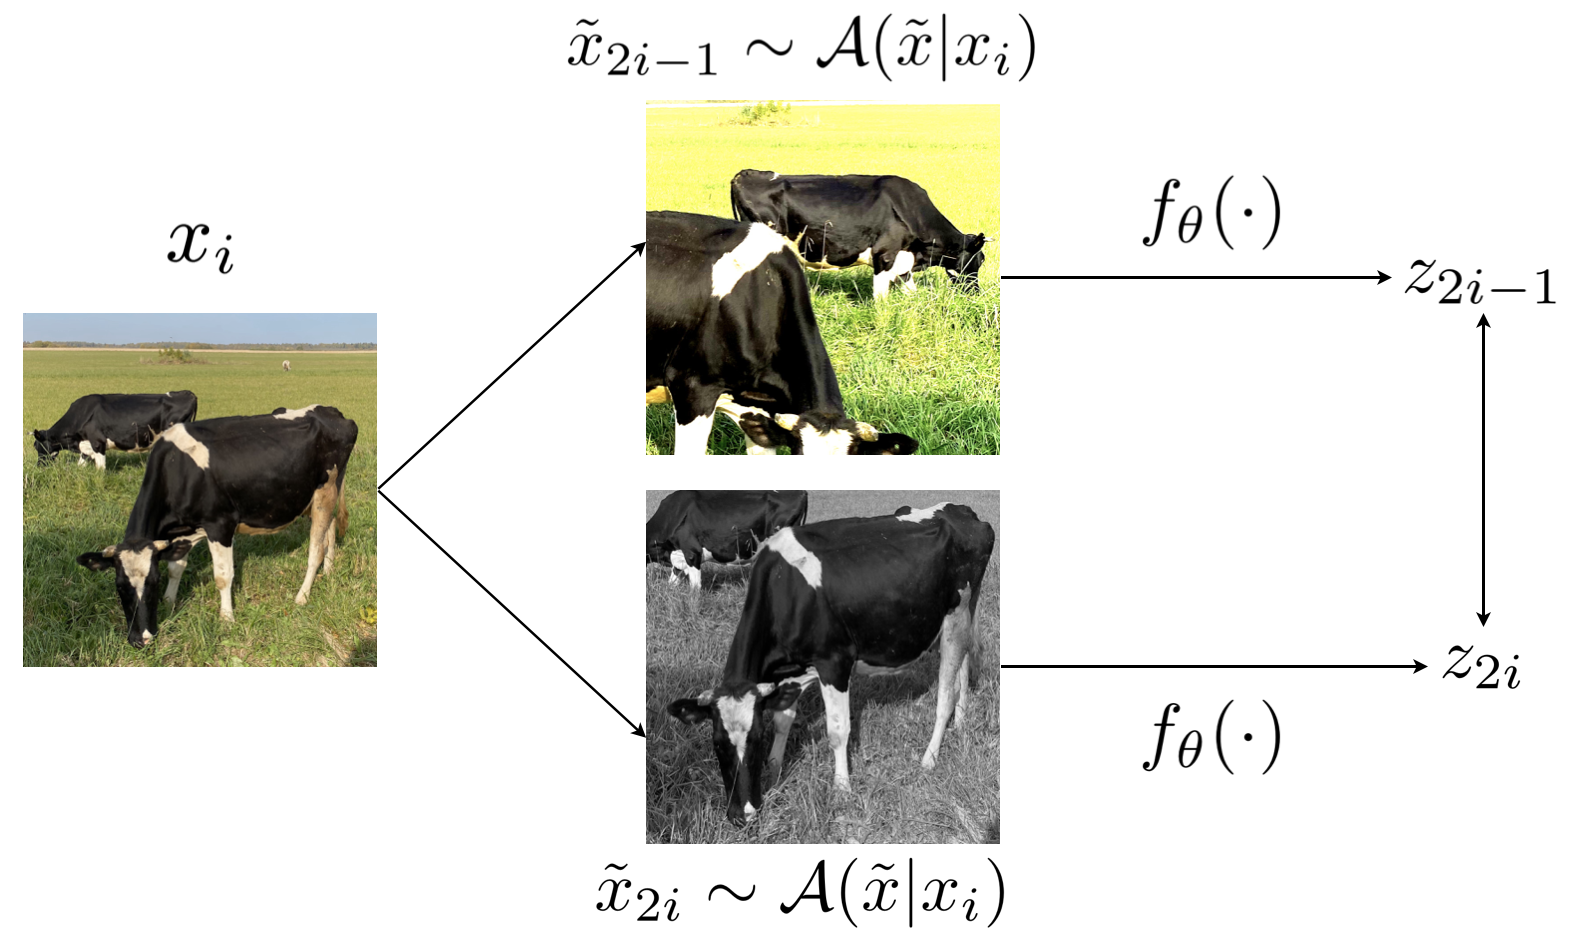
\includegraphics[width=14cm]{images/simclr.png}
    \caption{Схема работы метода SimCLR.}
    \label{simclr:pic:1}
\end{figure}{}

Пусть определена нейронная сеть $f_{\theta}: \R^{H \times W \times C} \rightarrow \R^d$, параметризованная весами $\theta \in \R^{\Theta}$, где $H \times W \times C$ --- размерности изображения, а $d$ --- размерность получаемого векторного представления. Рассмотрим один шаг обучения алгоритма на пакете изображений $\{x_i\}_{i=1}^B, x_i \in \R^{H \times W \times C}$ размера $B$. Пусть опредено некоторое распределение аугментаций $\mathcal{A}(\tilde{x}|x)$, зависящее от изображения $x$. Для каждого изображения $x_i$ из пакета метод генерирует две независимые случайные аугментации $\tilde{x}_{2i-1}, \tilde{x}_{2i} \sim \mathcal{A}(\tilde{x}|x_i)$. Затем данные аугментации пропускаются через нейронную сеть, на выходе получаются представления $z_{2i-1} = f_{\theta}(\tilde{x}_{2i-1})$ и $z_{2i} = f_{\theta}(\tilde{x}_{2i})$; $z_{2i-1}, z_{2i} \in \R^d$ (см. рис. \ref{simclr:pic:1}). Описанная процедура повторяется для всех изображений в пакете, на выходе имеем удвоенный пакет векторных представлений $\{z_{j}\}_{j=1}^B$, каждому изображению $x_i$ соответствуют два представления $z_{2i-1}$ и $z_{2i}$.

Для оптимизации параметров нейронной сети используется контрастная функция потерь \cite{contrastive}. Фактически, перед нейронной сетью ставится задача найти пару для каждого векторного представления. При этом среди всех представлений имеется один позитивный пример (собственно, представление парной аугментации изображения) и $2B-2$ негативных примера (все остальные представления). Определим вероятность $p(z_r|z_i)$ того, что представление $z_r$ соответствует представлению $z_i$:

\begin{equation}
    p(z_r|z_i) = \frac{\exp(\text{sim}(z_r, z_i)/\tau)}{\sum_{k=1}^{2B} [k \ne i] \exp(\text{sim}(z_k, z_i)/\tau)},
\end{equation}

\noindent
где $\text{sim}(u, v)$ --- некоторая функция похожести между векторами $u, v \in \R^d$ (в простейшем случае косинусное расстояние $\text{sim}(u, v) = u^T v /(\|u\|_2 \cdot \|v\|_2)$, $[k \ne i]$ - индикатор, равный 1 при $k \ne i$ и 0 в ином случае, а $\tau > 0$ --- гиперпараметр температуры. По сути, вероятность $p(z_r|z_i)$ задается через оператор softmax на похожестях векторных представлений, что задает дискретное вероятностное распределение на представлениях. Наряду с этим, для каждого представления задан истинный класс ($z_{2k-1}$ для $z_{2k}$ и $z_{2k}$ для $z_{2k-1}$), а остальные $2B-2$ класса являются ложными. Таким образом, метод SimCLR можно рассматривать как классификацию представлений внутри одного пакета, а контрастная функция потерь $\mathcal{L}(\theta, \{x_k\}_{k=1}^B)$ получается эквивалентной кросс-энтропийной функции потерь:
\begin{equation}
    \mathcal{L}(\theta, \{x_k\}_{k=1}^B) = -\frac{1}{2B} \sum_{k=1}^B \Big(\log p(z_{2k}|z_{2k-1}) + \log p(z_{2k-1}|z_{2k})\Big)
\end{equation}

\noindent
Оптимизационный процесс рассчитан на минимизацию мат. ожидания контрастной функции потерь по распределению обучающей выборки $\mathcal{D}$:
\begin{equation}
    \E_{\{x_k\}_{k=1}^B \sim \mathcal{D}} \Big[ \mathcal{L}(\theta, \{x_k\}_{k=1}^B) \Big] \rightarrow \min_{\theta}
\end{equation}


\section{Эксперименты}
В экспериментах мы сравниваем три различных постановки: алгоритм SimCLR как self-supervised learning метод, обучение с учителем на примере классификации изображений и обучение со случайной разметкой по классам. В качестве случайной разметки используется фиксированная случайная перестановка классов обучающих объектов, что позволяет сохранить исходный баланс классов. Эксперименты проводятся на наборе данных CIFAR-10 \cite{cifar}, используется архитектура сверточной нейронной сети ResNet-18 \cite{resnet}. Аугментации изображений играют значимую роль в первых двух постановках, поэтому обучение со случайной разметкой мы рассматриваем в двух вариациях: с использованием аугментаций и без них. При этом в алгоритме SimCLR применяются более интенсивные аугментации, чем при обучении с учителем. При обучении со случайной разметкой используются те же аугментации, что и при обучении с учителем. Более подробное описание типов аугментаций, а также других гиперпараметров обучения доступно в \hyperref[appendix:1]{Приложении А}.

Наши эксперименты устанавливают, как меняются предсказания нейронных сетей по ходу обучения. Кроме того, мы проверяем, что обуславливает сложность выучивания тех или иных объектов. Мы устанавливаем, что сами объекты обладают неодинаковой сложностью в контексте рассмотренных постановок обучения. Вдобавок мы изучаем влияние аугментаций на сложность объектов и показываем, что аугментации в методе SimCLR увеличивают разброс сложности объектов (то есть выделяются очень простые и очень сложные изображения), в то время как сложности, ассоциированные с самими объектами, являются более однородными.

\subsection{Динамика обучения}

Наш подход к изучению динамики обучения вдохновлен \cite{memorization}. В \hyperref[simclr:1]{разделе 3} показано, что алгоритм SimCLR эквивалентен задаче классификации внутри пакета размера $B$ с $2B-1$ классом. Таким образом, все упомянутые постановки представляют собой задачи классификации. Рассмотрим нейронную сеть $f_{\theta}: \R^{H \times W \times C} \rightarrow [0, 1]^L$, параметризованную весами $\theta \in \R^{\Theta}$, которая предсказывает вероятности $L$ классов. Пусть вероятность класса $y \in \{1, \dots, L\}$ для изображения $x \in \R^{H \times W \times C}$ обозначается как $p_{\theta}(y|x)$, $\sum_{y=1}^L p_{\theta}(y|x)=1$. Пусть также $y_{\text{true}}$ --- истинный класс изображения $x$. Тогда событие $y_{\text{true}} = \argmax_{y} p_{\theta}(y|x)$ означает, верно ли изображение $x$ классифицировано нейронной сетью $f_{\theta}$.

Рассмотрим теперь $\theta \sim \mathcal{T}(t)$ --- распределение весов нейронной сети $f_{\theta}$ после $t$ эпох обучения (здесь в случайность входит начальная инициализация, перемешивание объектов стохастического градиентного спуска и аугментации изображений обучающей выборки). Напомним также, что $\mathcal{A}(\tilde{x}|x)$ обозначает распределение аугментаций изображения $x$. Центральной величиной является $r_t(x)$ --- вероятность того, что аугментированное изображение $x$ правильно классифицируется после $t$ эпох обучения:
\begin{equation}
    r_t(x) = \mathbb{P}_{\substack{\theta \sim \mathcal{T}(t) \\ \tilde{x} \sim \mathcal{A}(\tilde{x}|x)}} \Big(y_{\text{true}} = \argmax_{y} p_{\theta}(y|\tilde{x})\Big)
\end{equation}

Мы переписываем вероятность события как мат. ожидание индикатора и оцениваем его методом Монте-Карло, обучая несколько копий нейронной сети из разных начальных инициализаций:
\begin{equation}
\label{experiments:eq:1}
\begin{gathered}
    r_t(x) = \E_{\substack{\theta \sim \mathcal{T}(t) \\ \tilde{x} \sim \mathcal{A}(\tilde{x}|x)}} \Big[\big[y_{\text{true}} = \argmax_{y} p_{\theta}(y|\tilde{x})\big]\Big] \approx \\
    \approx \frac{1}{NM} \sum_{i=1}^N\sum_{j=1}^M \big[y_{\text{true}} = \argmax_{y} p_{\theta_i}(y|\tilde{x}_j)\big],
\end{gathered}
\end{equation}

\noindent
где $N$ --- число копий нейронной сети, $\theta_i \sim \mathcal{T}(t)$ --- веса одной копии, \linebreak $M$ --- число аугментаций, $\tilde{x}_j \sim \mathcal{A}(\tilde{x}|x)$ --- одна аугментация изображения. В экспериментах используются значения $N=30, M=10$.

Мы анализируем динамику обучения различных постановок, оценивая величину $r_t(x)$ на некоторой фиксированной подвыборке обучающих объектов. При этом для каждого алгоритма используется то же самое распределение аугментаций, что и при обучении (в частности, при обучении со случайной разметкой аугментации не используются, а значит, распределение аугментаций в этом случае вырождается в дельта-распределение в точке исходного изображения: $\mathcal{A}(\tilde{x}|x) = \delta(\tilde{x} - x)$).

\begin{figure}[H]
    \centering
    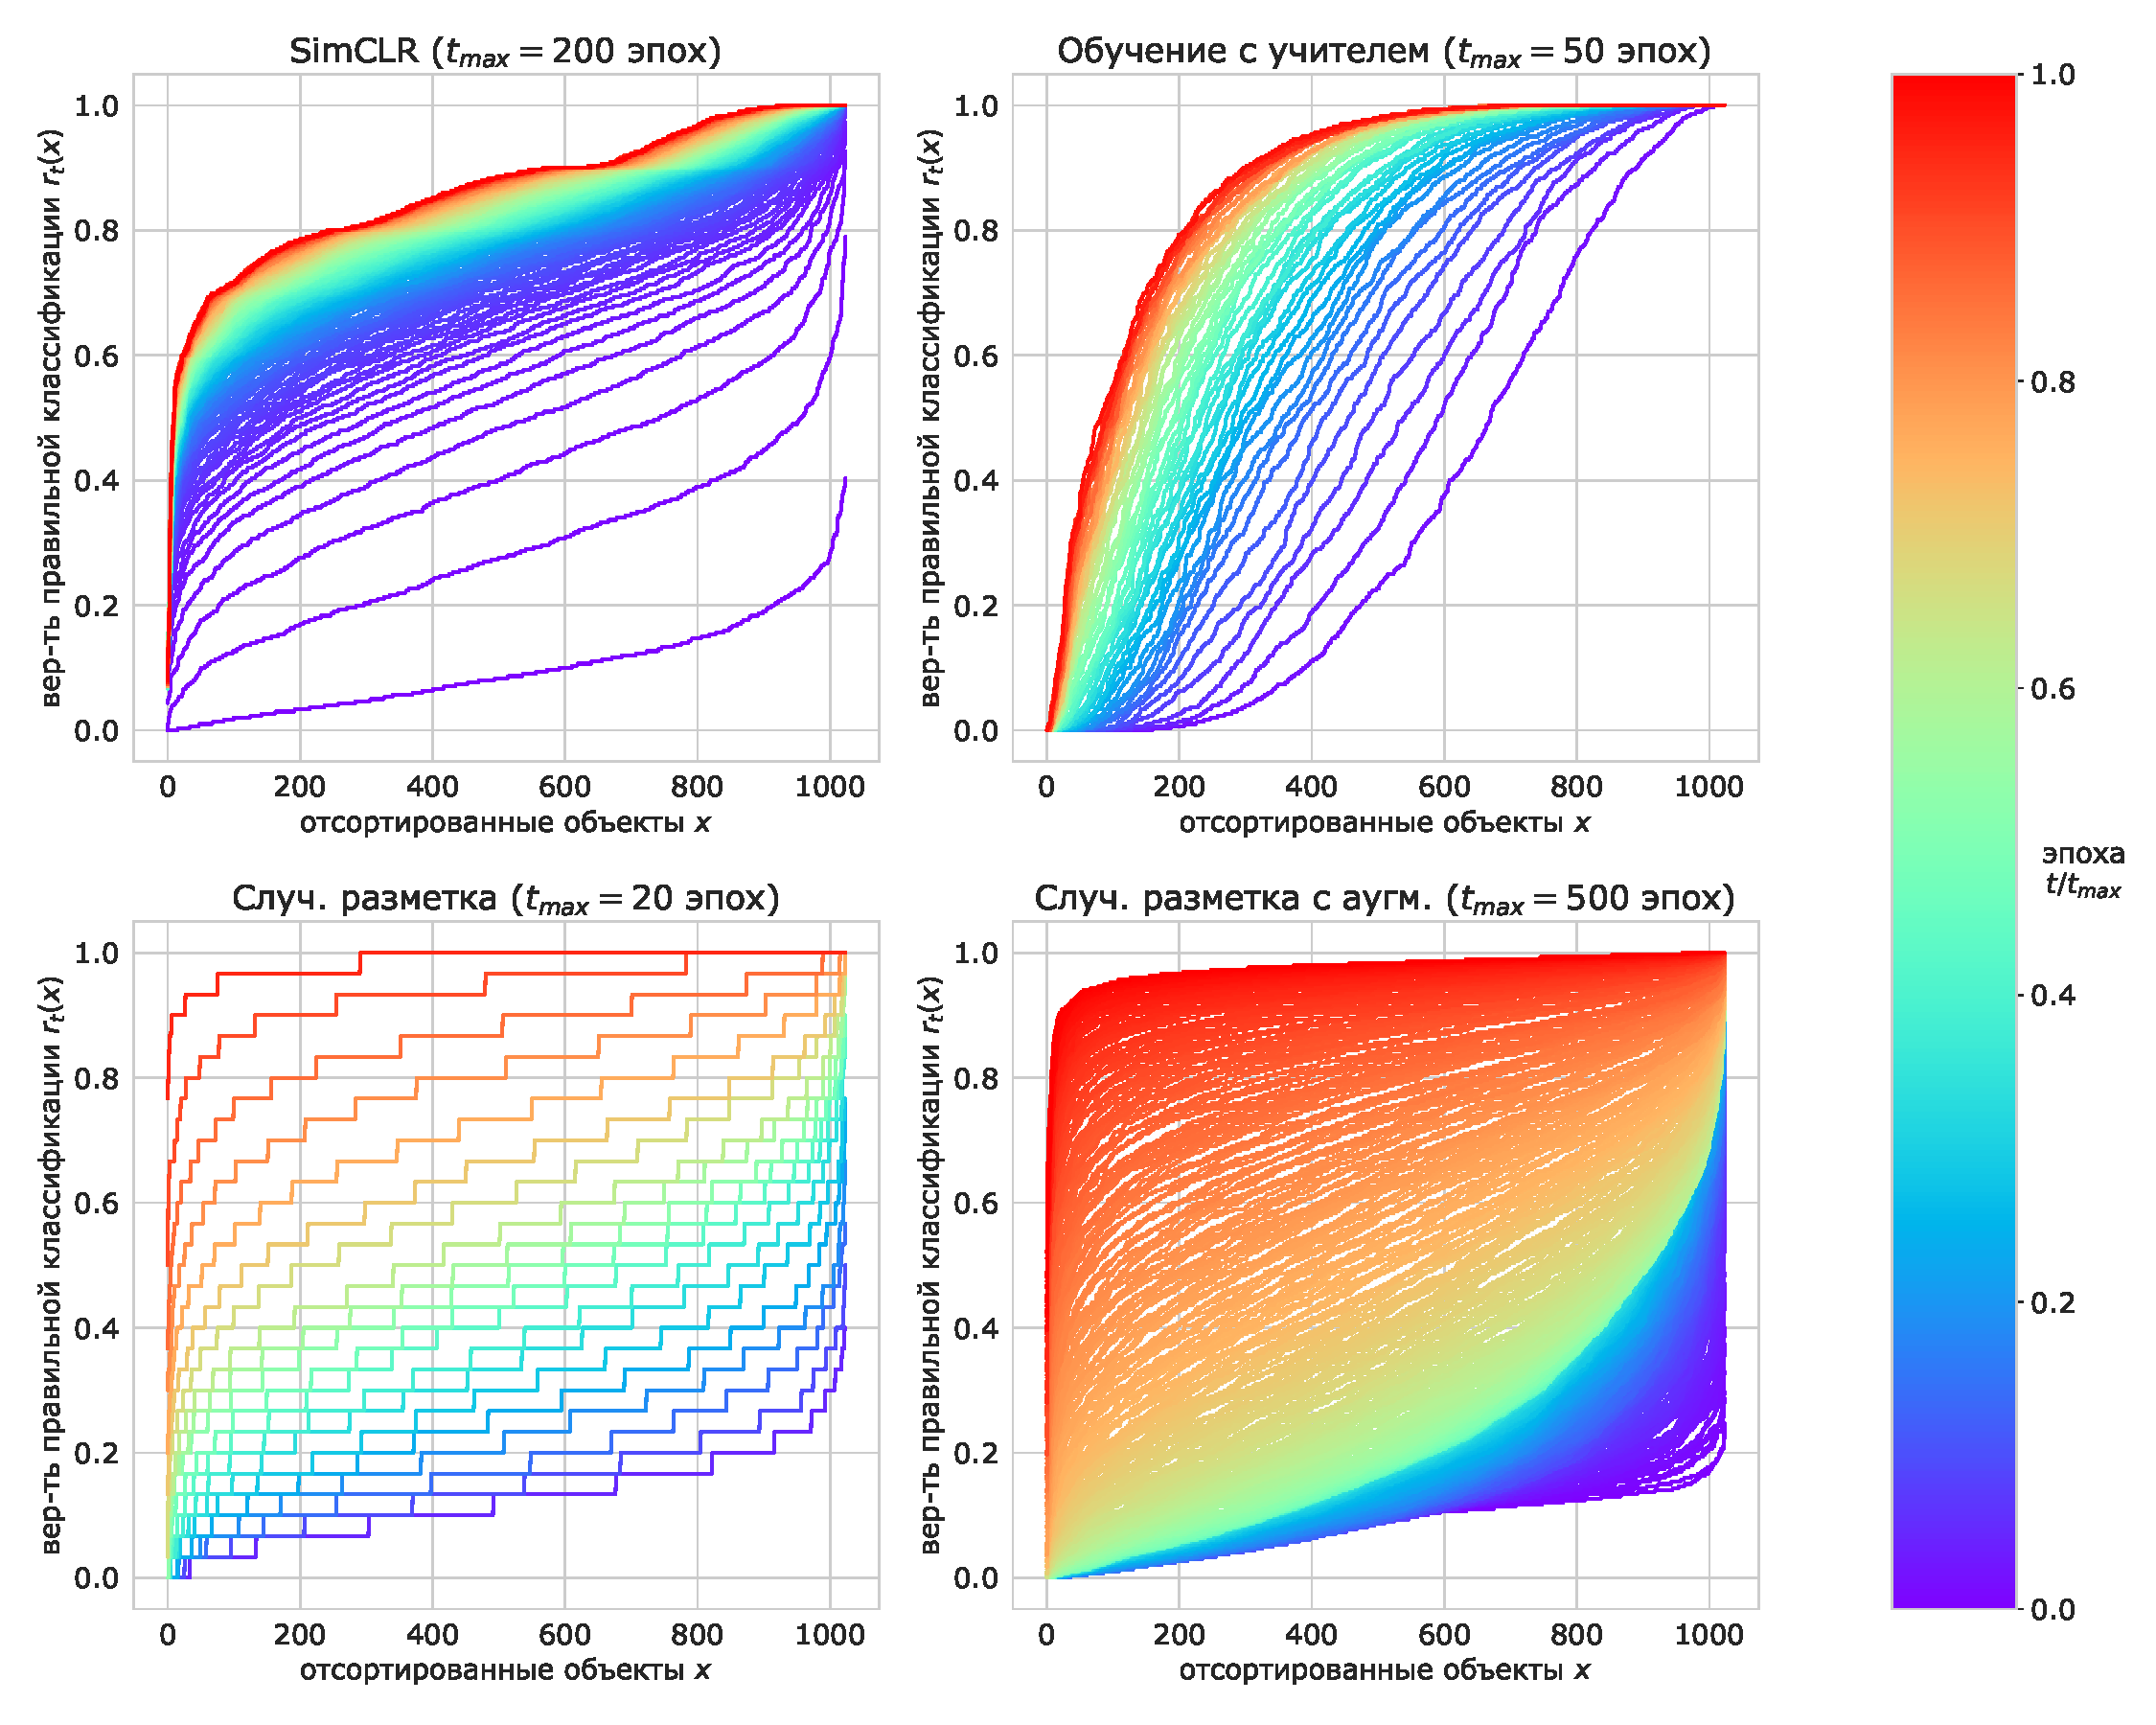
\includegraphics[width=17cm]{images/training_dynamics.pdf}
    \caption{Динамика обучения различных методов. По горизонтальной оси отложены объекты из обучающей подвыборки размера $K=1024$, отсортированные по величине $r_t(x)$ независимо по эпохам, по вертикальной оси - показатель $r_t(x)$. Цвет линии для каждой эпохи $t$ выставлен относительно максимального числа эпох $t_{\max}$ (своё для каждого метода). Ввиду отсутствия усреднения по аугментациям рисунок для обучения со случайной разметкой имеет характерный ступенчатый вид с высотой ступеней 1/N.}
    \label{experiments:pic:1}
\end{figure}{}

Также стоит отметить, что в методе SimCLR для каждого изображения $x$ есть по две отдельные задачи классификации, так как используются две его аугментации $\tilde{x}_1, \tilde{x}_2 \sim \mathcal{A}(\tilde{x}|x)$. Соответственно, для аугментации $\tilde{x}_1$ правильным классом является $\tilde{x}_2$, и наоборот. Условные вероятности $p_{\theta}(\tilde{x}_2|\tilde{x}_1)$ и $p_{\theta}(\tilde{x}_1|\tilde{x}_2)$, вообще говоря, не равны. Индикаторы для $\tilde{x}_1$ и $\tilde{x}_2$ из ур. \ref{experiments:eq:1} также могут отличаться, отчего не ясно, какой именно индикатор подставлять в формулу $r_t(x)$. Однако наличие усреднения по аугментациям решает данную проблему (не имеет значения, какой из двух индикаторов использовать), что подтверждается дополнительными материалами, изложенными в \hyperref[appendix:2]{Приложении Б}.

На рис. \ref{experiments:pic:1} показана эволюция величины $r_t(x)$ различных методов от начальных и до финальных эпох обучения. Кривая для каждой эпохи представляет собой отсортированные значения $r_t(x)$. Однако рассмотренные методы имеют разную скорость обучения, поэтому максимальное число эпох $t_{\max}$ своё у каждого метода. Данный график демонстрирует, что методы имеют непохожее распределение $r_t(x)$, особенно выделяются кривые обучения с учителем, имеющие s-образную форму на ранних стадиях обучения. Дальнейший анализ направлен на более подробное сравнение методов.

Как уже обсуждалось выше, методы имеют разную скорость обучения, поэтому для справедливого сравнения их необходимо уравнять по эпохам. Пусть $\mathcal{D}$ --- это распределение изображений обучающей выборки. Мы предлагаем сопоставлять эпохи обучения друг другу по величине $\E_{x \sim \mathcal{D}} \big[r_t(x)\big]$ --- средней по обучающим объектам вероятности правильной классификации. Данную величину мы также оцениваем методом Монте-Карло по обучающей подвыборке размера $K=1024$:
\begin{equation}
    \E_{x \sim \mathcal{D}} \big[r_t(x)\big] \approx \frac{1}{K} \sum_{k=1}^K r_t(x_k)
\end{equation}

\noindent
Данная оценка приближенно совпадает с площадью под отсортированной кривой $r_t(x)$, как на рис. \ref{experiments:pic:1}. Из графика следует, что площадь под кривой растет по ходу обучения, поэтому уравнивать алгоритмы по указанному показателю представляется разумным.

Далее, рассмотрим два алгоритма обучения $A$ и $B$. Зафиксируем число эпох обучения алгоритма A как $t_A$. Тогда соответствующее ему число эпох $t_B$ алгоритма $B$ определяется как:
\begin{equation}
    t_B = \argmin_t \Big|\E_{x \sim \mathcal{D}} \big[r^A_{t_A}(x)\big] - \E_{x \sim \mathcal{D}} \big[r^B_{t}(x)\big]\Big|,
\end{equation}

\noindent
где величина $r^A_{t}(x)$ относится к алгоритму $A$, а $r^B_{t}(x)$ --- к алгоритму $B$. Поскольку данные для оценки $r_t(x)$ собираются в дискретные моменты времени обучения (раз в эпоху), то достичь точного равенства мат. ожиданий не удается, но описанная эвристика позволяет сопоставить стадии обучения различных методов.

\begin{figure}[H]
    \centering
    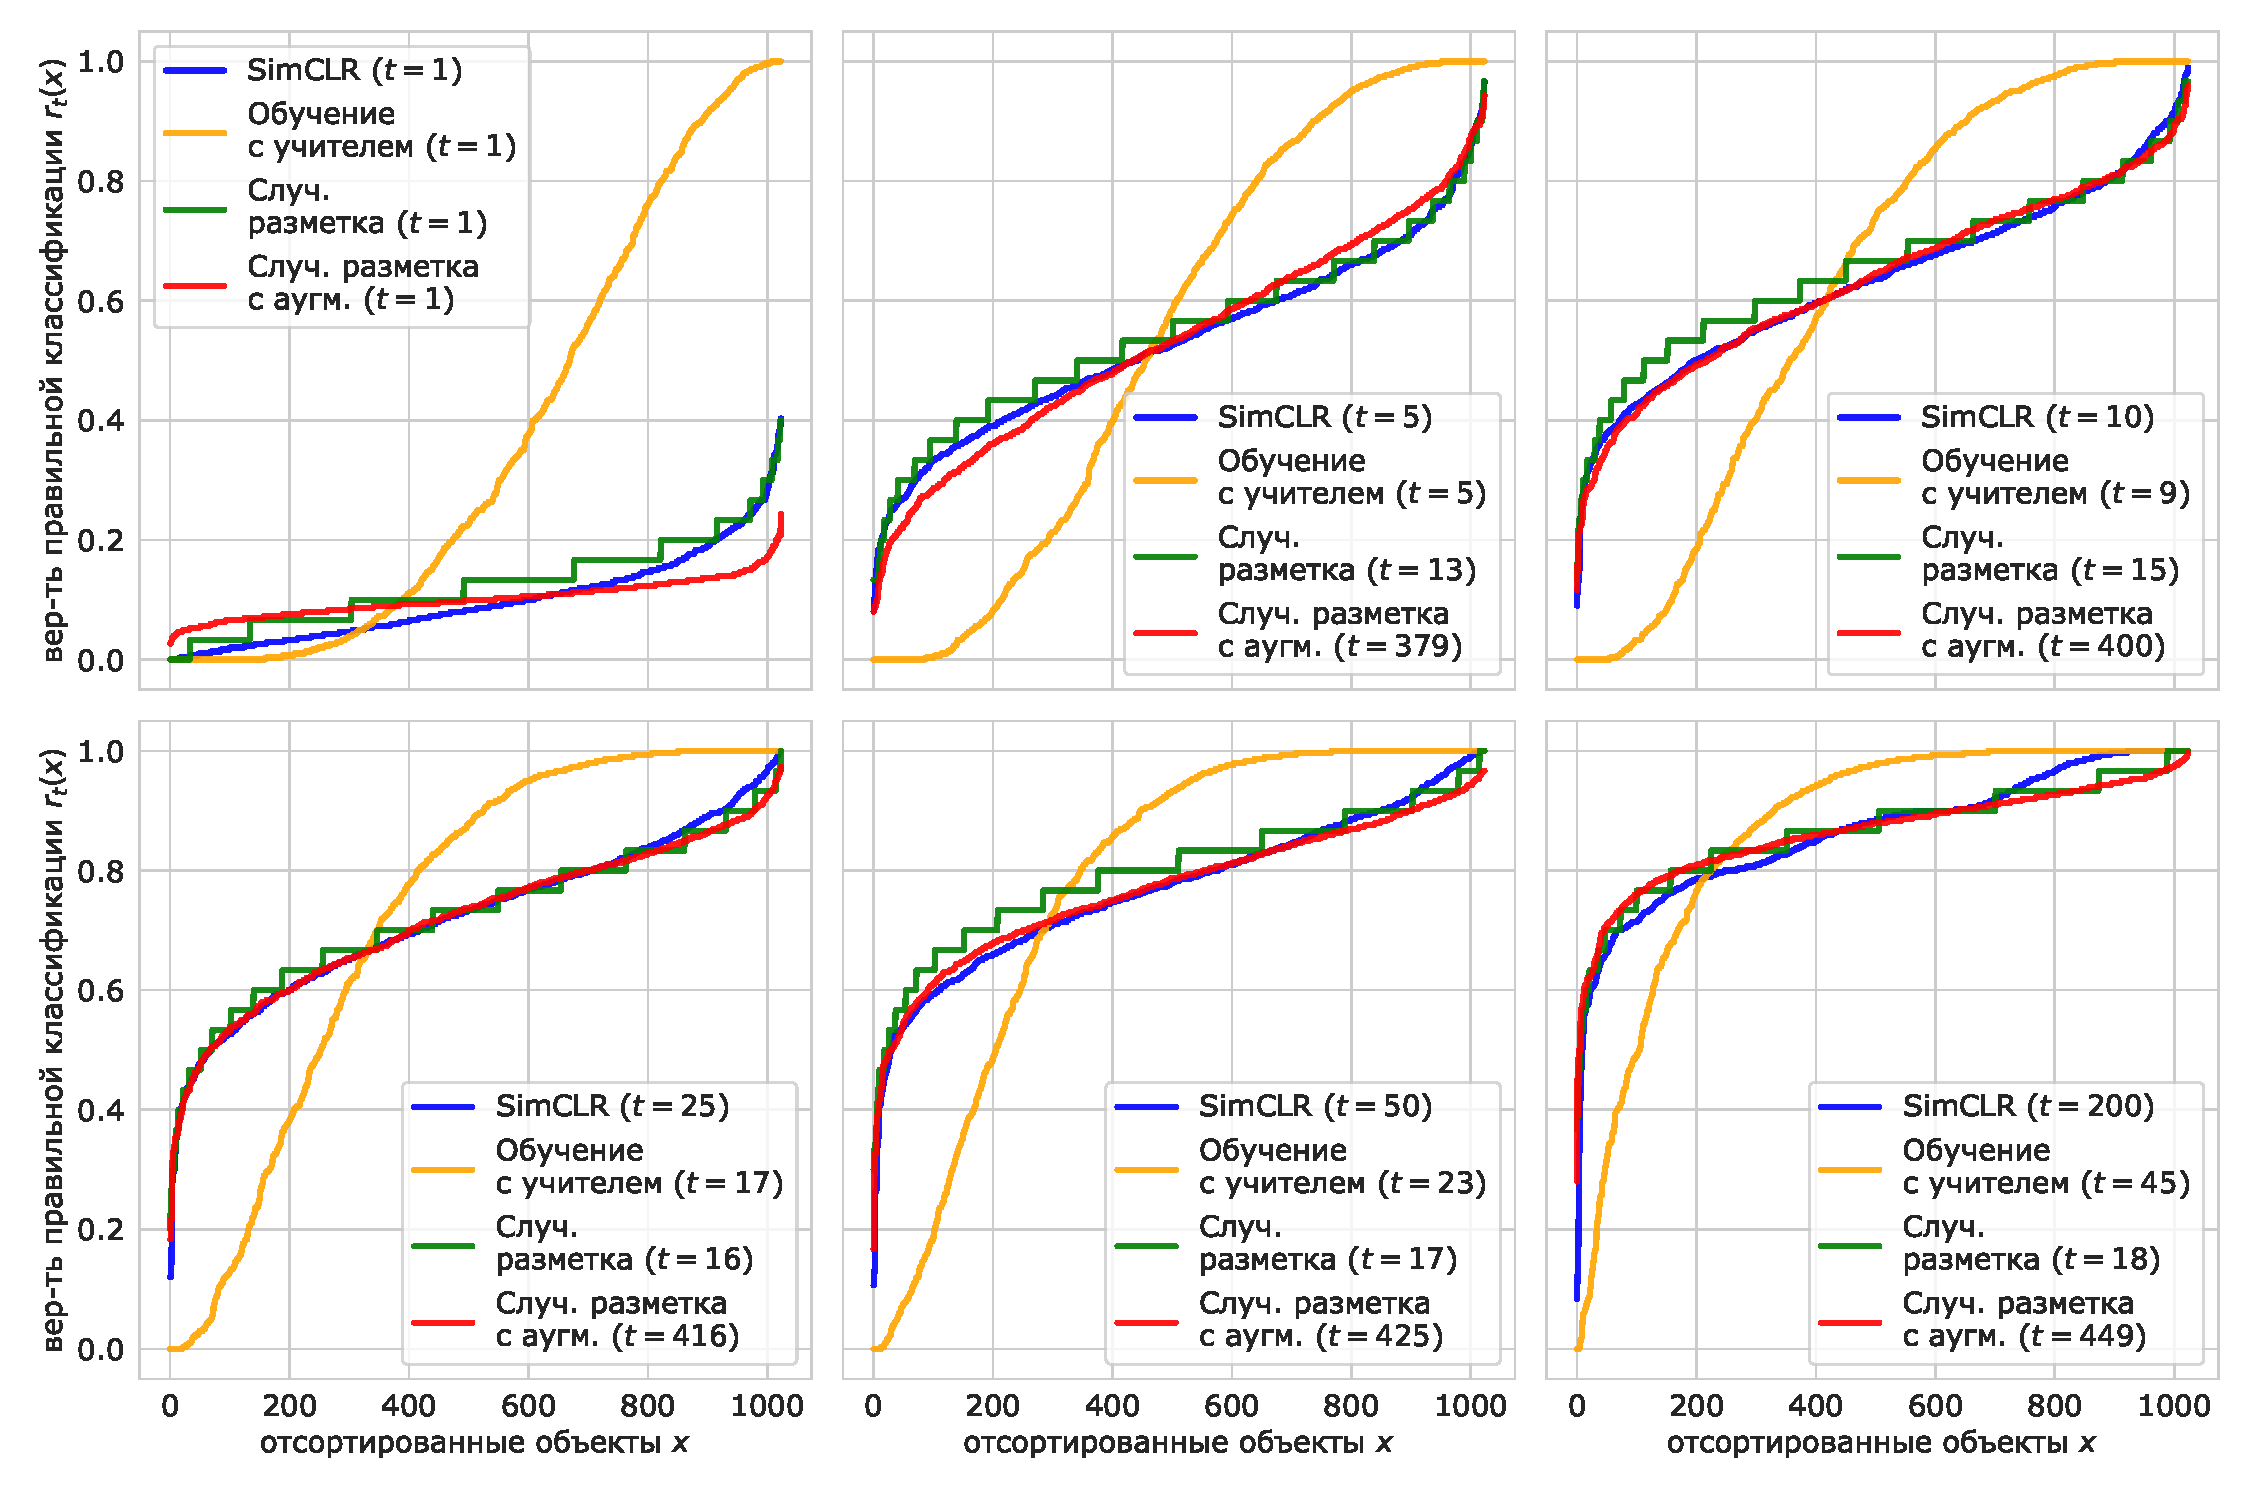
\includegraphics[width=17cm]{images/equal_areas.pdf}
    \caption{Сравнение динамики обучения методов. Обозначения в скобках показывают число эпох $t$ обучения при подсчете величины $r_t(x)$.}
    \label{experiments:pic:2}
\end{figure}{}

На рис. \ref{experiments:pic:2} представлен результат сравнения динамики обучения алгоритмов с учетом выравнивания по эпохам. Опорным методом для сопоставления эпох выбран SimCLR, рассмотрены значения $t \in \{1, 5, 10, 25, 50, 200\}$. Неожиданным выводом здесь оказывается, что динамика обучения метода SimCLR очень похожа на динамику обучения со случайной разметкой. Мы предлагаем следующую интуицию, объясняющую данный феномен: в обеих постановках нейронная сеть должна научиться непосредственно распознавать изображения обучающей выборки. В случае метода SimCLR каждое изображение, по сути, является отдельным классом, а аугментации изображения - примерами класса. При обучении со случайной разметкой последняя не несет никакой информации об объектах, так что для правильной классификации обучающей выборки от нейронной сети требуется запомнить все обучающие примеры. При обучении с учителем, напротив, разметка является информативной, и нейронной сети достаточно выделить фрагменты изображений, специфичные для каждого класса, отчего нет необходимости заучивать обучающую выборку, что и приводит к другой форме кривой $r_t(x)$.

\subsection{Сравнение с биномиальным шумом}
\label{experiments:1}

Следующая серия экспериментов проверяет гипотезу о простых и сложных объектах, сформулированную в \cite{memorization}: нейронные сети выучивают некоторые объекты обучающей выборки быстрее, чем остальные. Предположим, что гипотеза не верна, и все обучающие объекты $x$ имеют одинаковую сложность. Тогда случайная величина $[y_{\text{true}} = \argmax_{y} p_{\theta}(y|x)]$ зависит от распределения $\theta \sim \mathcal{T}(t)$, но не от $x \sim \mathcal{D}$. Поскольку индикатор принимает бинарные значения, то можно считать, что он имеет распределение Бернулли с некоторой вероятностью $p_0$, не зависящей от объекта $x$. Индикатор зависит только от $\theta$, поэтому при независимых $\theta_1, \theta_2 \sim \mathcal{T}(t)$ соответствующие им индикаторы также будут независимыми.

Теперь для каждого изображения $x$ зафиксируем его случайную аугментацию $\tilde{x} \sim \mathcal{A}(\tilde{x}|x)$ и рассмотрим величину $\tilde{r}_t(\tilde{x})$:
\begin{equation}
\begin{gathered}
    \tilde{r}_t(\tilde{x}) = \mathbb{P}_{\theta \sim \mathcal{T}(\theta)} \Big(y_{\text{true}} = \argmax_{y} p_{\theta}(y|\tilde{x})\Big) = \\
    = \E_{\theta \sim \mathcal{T}(t)} \Big[\big[y_{\text{true}} = \argmax_{y} p_{\theta}(y|\tilde{x})\big]\Big] \approx \frac{1}{N} \sum_{i=1}^N [y_{\text{true}} = \argmax_{y} p_{\theta_i}(y|\tilde{x})]
\end{gathered}
\end{equation}

\noindent
Фактически, $\tilde{r}_t(\tilde{x})$ отличается от рассмотренной выше $r_t(x)$ отсутствием \linebreak усреднения по аугментациям. Итак, если все аугментированные изображения имеют одинаковую сложность, то случайная величина $\tilde{r}_t(\tilde{x})$ распределена биномиально с точностью до константы $1/N$ (как сумма независимых бернуллиевских случайных величин):
\begin{equation}
\begin{gathered}
    \tilde{r}_t(\tilde{x}) \approx \frac{1}{N} \sum_{i=1}^N [y_{\text{true}} = \argmax_{y} p_{\theta_i}(y|\tilde{x})] \sim \frac{1}{N} \sum_{i=1}^N \text{Bern}(p_0) = \\
    = \frac{1}{N} \text{Bin}(N, p_0)
\end{gathered}
\end{equation}

Далее, для каждого метода обучения мы предлагаем проверить нулевую гипотезу, что случайная величина $N \tilde{r}_t(\tilde{x})$ имеет биномиальное распределение $\text{Bin}(N, \widehat{p}_0(t))$. Для этого мы оцениваем параметр $\widehat{p}_0(t)$ по выборке:
\begin{equation}
    \widehat{p}_0(t) = \frac{1}{K} \sum_{k=1}^K \tilde{r}_t (\tilde{x}_k) 
\end{equation}

\noindent
Для проверки гипотезы используется хи-квадрат тест равенства частот \cite{chisquare}. При этом число степеней свободы распределения хи-квадрат уменьшается на 1 за счет оценивания по данным одного параметра $\widehat{p}_0(t)$.

Чтобы не проводить тестирование гипотезы для каждой эпохи обучения, мы выделяем по 3 эпохи на каждый алгоритм. Для $p_0 \in [0.25, 0.5, 0.75]$ мы выбираем первую по порядку эпоху $t$, при которой $\widehat{p}_0(t) > p_0$. Таким образом, всего проверяется 12 гипотез --- для каждой из 3 эпох по 4 алгоритмам.

\begin{figure}[H]
    \centering
    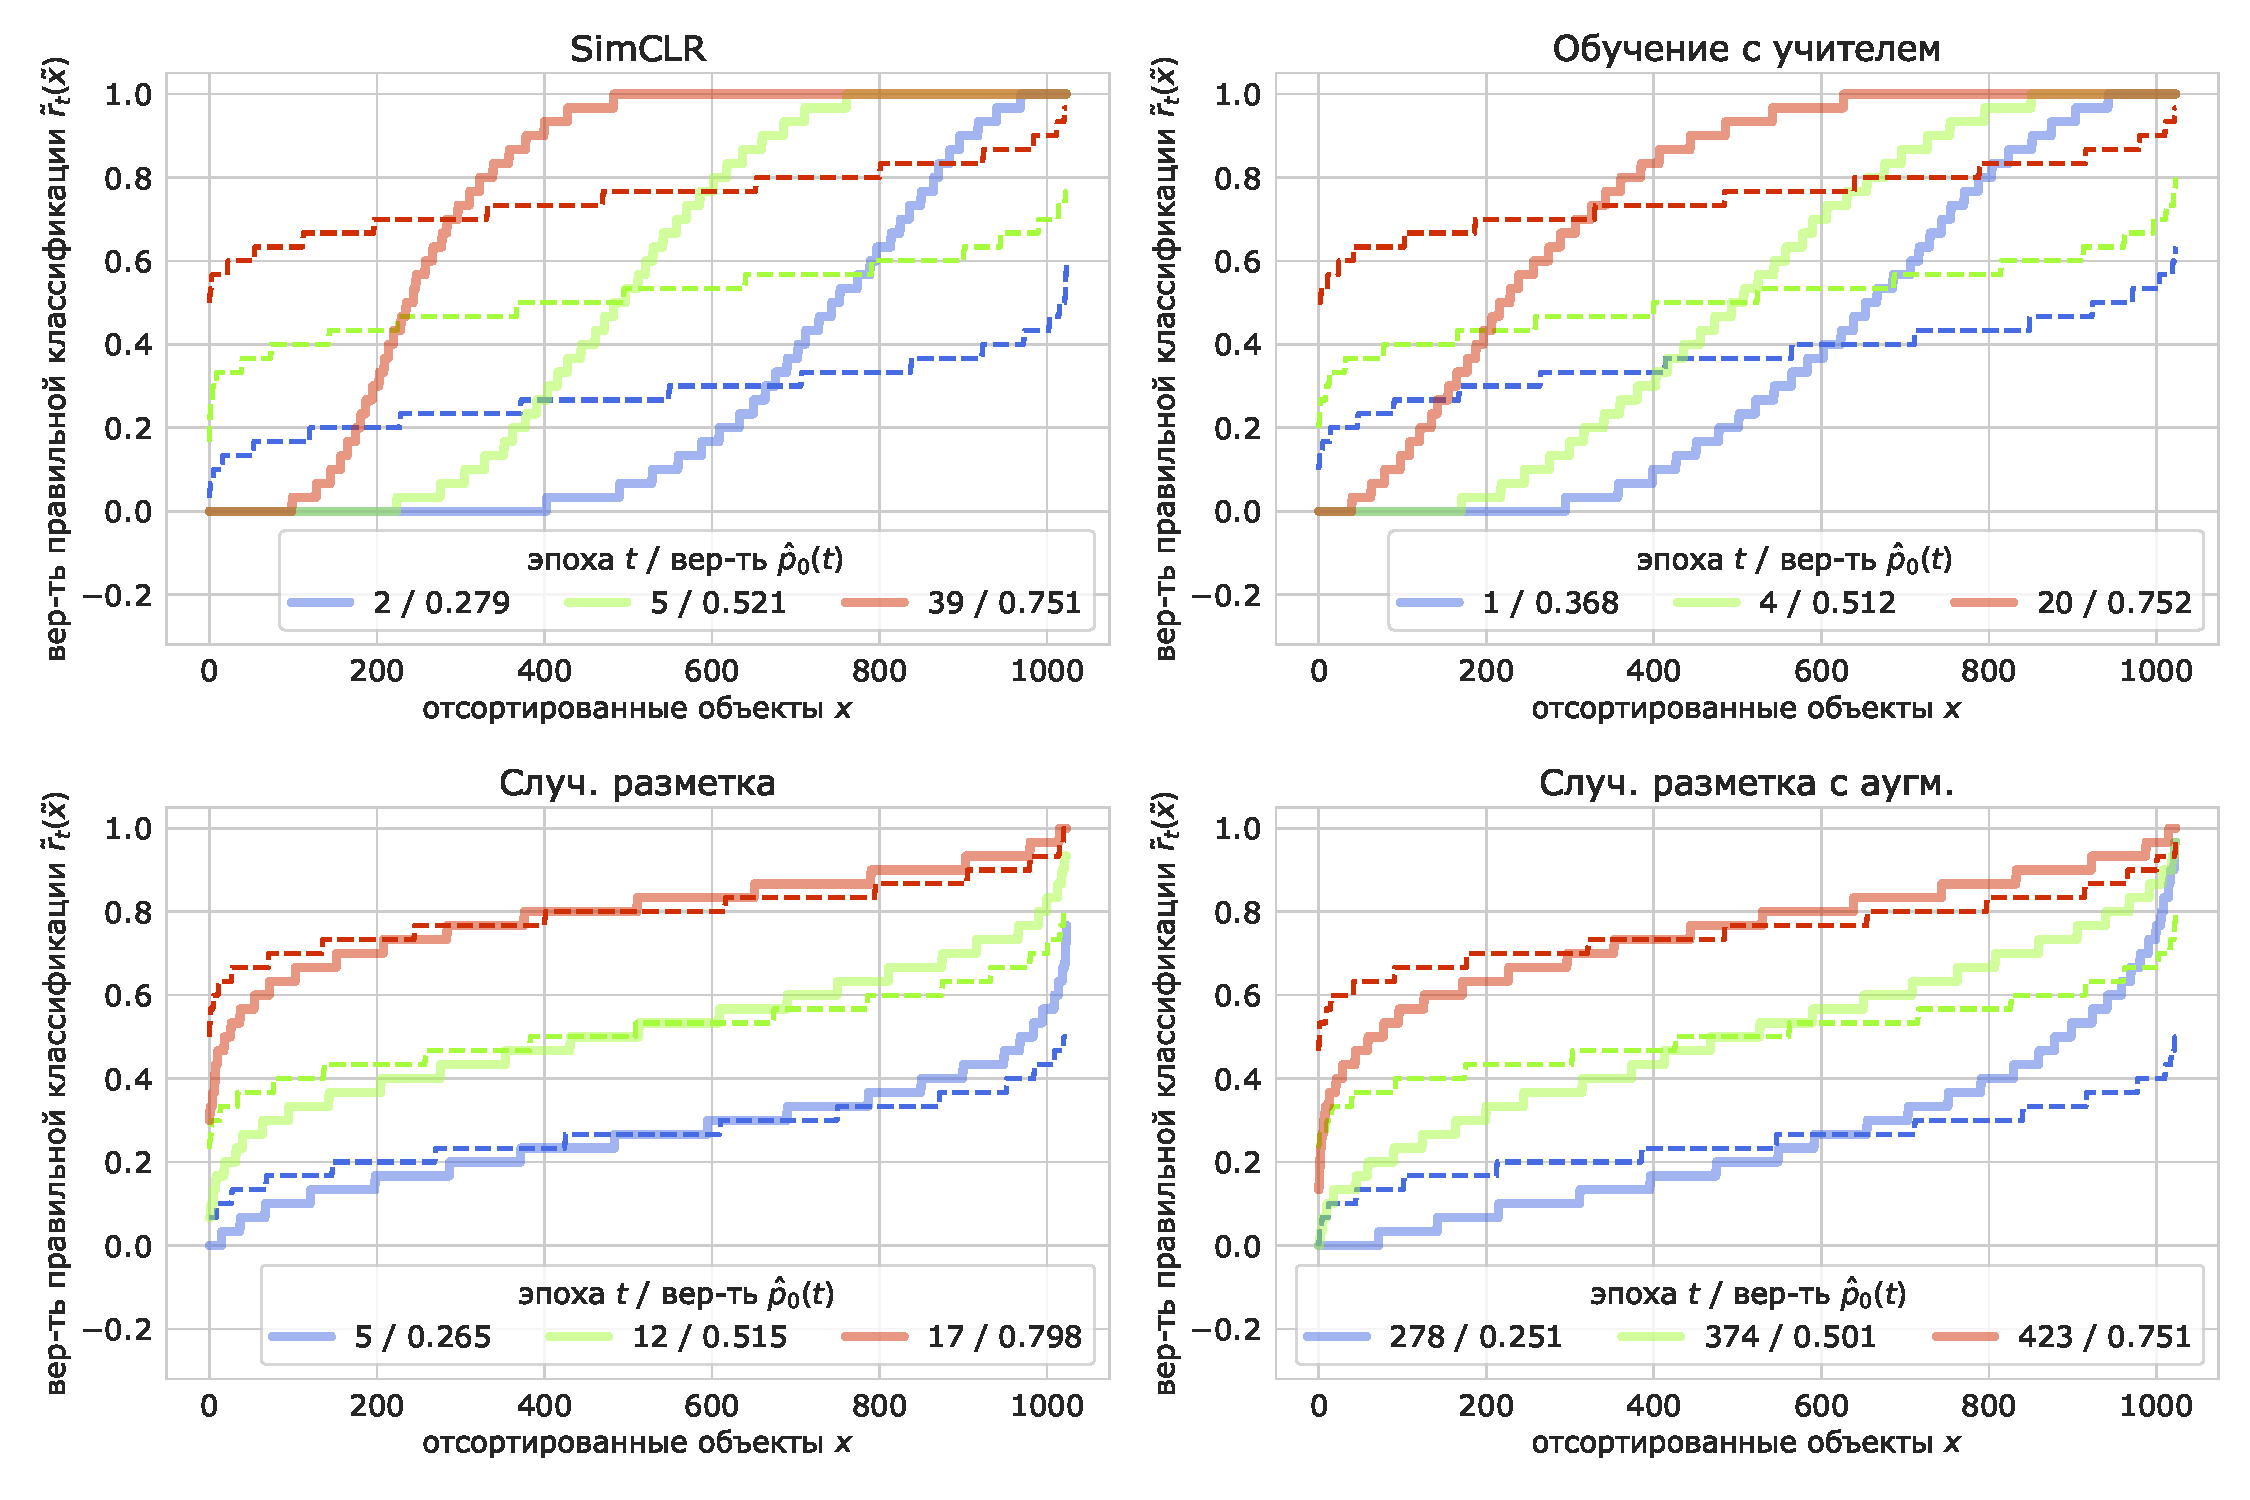
\includegraphics[width=17cm]{images/binom_noise1.pdf}
    \caption{Сравнение величины $\tilde{r}_t(\tilde{x})$ (сплошная жирная линия) с соответствующим биномиальным шумом (пунктирная линия).}
    \label{experiments:pic:3}
\end{figure}{}

Из рис. \ref{experiments:pic:3} становится очевидно, что нулевая гипотеза не верна. Это же подтверждается и результатами теста, приведенными в таблице \ref{experiments:table:1}. Таким образом, аугментированные изображения имеют разную сложность в контексте всех четырех алгоритмов. Тем не менее, нельзя не отметить, что распределение $\tilde{r}_t(\tilde{x})$ обучения со случайной разметкой больше всего напоминает биномиальное: это заметно и по графикам, и по меньшим значениям тестовой статистики $\chi^2$. Данное наблюдение свидетельствует о том, что при обучении со случайной разметкой объекты имеют меньший разброс сложности. Напротив, при отсутствии усреднения по аугментациям кривые метода SimCLR становятся похожи на кривые обучения с учителем. Данные кривые сильно отличаются от биномиального шума, то есть присутствуют как очень простые, так и очень сложные объекты. Мы предполагаем, что конкретные аугментации увеличивают разброс сложности объектов, и потому проводим похожий эксперимент с добавлением усреднения по аугментациям.

\begin{table}[H]
    \centering
    \begin{tabular}{|C{2.5cm}|C{1.75cm}|C{2.75cm}|C{3.25cm}|C{2.75cm}|}
        \hline
        Метод & Эпоха $t$ & Вер-ть $\widehat{p}_0(t)$ & Тест. статистика $\chi^2$ & P-значение \\ \hline
        \multirow{3}{*}{SimCLR} & 2 & 0.279 & $1.3 \cdot 10^{17}$ & 0.0 \\ \cline{2-5}
        & 5 & 0.521 & $2.1 \cdot 10^{11}$ & 0.0 \\ \cline{2-5}
        & 39 & 0.751 & $1.3 \cdot 10^{19}$ & 0.0 \\ \hline
        \multirow{3}{*}{\shortstack{Обучение\\с учителем}} & 1 & 0.368 & $6.7 \cdot 10^{13}$ & 0.0 \\ \cline{2-5}
        & 4 & 0.512 & $8 \cdot 10^{10}$ & 0.0 \\ \cline{2-5}
        & 20 & 0.752 & $2.4 \cdot 10^{18}$ & 0.0 \\ \hline
        \multirow{3}{*}{\shortstack{Случ.\\разметка}} & 5 & 0.265 & $8.4 \cdot 10^{4}$ & 0.0 \\ \cline{2-5}
        & 12 & 0.515 & $4.2 \cdot 10^{4}$ & 0.0 \\ \cline{2-5}
        & 17 & 0.798 & $4.5 \cdot 10^{5}$ & 0.0 \\ \hline
        \multirow{3}{*}{\shortstack{Случ.\\разметка\\с аугм.}} & 278 & 0.251 & $4.4 \cdot 10^{13}$ & 0.0 \\ \cline{2-5}
        & 374 & 0.501 & $5.2 \cdot 10^{6}$ & 0.0 \\ \cline{2-5}
        & 423 & 0.751 & $5.9 \cdot 10^{8}$ & 0.0 \\ \hline
    \end{tabular}
    \caption{Результаты хи-квадрат теста. Все нулевые гипотезы и так отклоняются, поэтому поправка на множественное тестирование гипотез не требуется.}
    \label{experiments:table:1}
\end{table}

Мы расширяем анализ на величину $r_t(x)$, чтобы исключить влияние аугментаций на сложность объектов. Усреднение по аугментациям заметно усложняет теоретический вывод. Ур. \ref{experiments:eq:1} можно переписать в следующем виде:
\begin{equation}
    r_t(x) \approx \frac{1}{N} \sum_{i=1}^N \bigg( \frac{1}{M} \sum_{j=1}^M \big[y_{\text{true}} = \argmax_{y} p_{\theta_i}(y|\tilde{x}_j)\big] \bigg)
\end{equation}

\noindent
Из-за наличия зависимостей между аугментациями одного изображения слагаемое в скобках уже нельзя представить в виде простого распределения (получается некоторое дискретное распределение на множестве $\{0, 1/M, \dots, 1\}$). Мы предлагаем провести менее формальный анализ, приняв биномиальное распределение за образец однородной сложности объектов. В качестве метрики мы используем среднюю абсолютную ошибку (англ. mean absolute error, MAE) между отсортированными кривыми $r_t(x)$ (приблизительно равна площади между кривыми):
\begin{equation}
    \text{MAE}\Big(\{x_k\}_{k=1}^K, \{b_k\}_{k=1}^K\Big) = \frac{1}{K} \sum_{k=1}^K |r_t(x_k) - b_k|,
\end{equation}

\noindent
где значения $r_t(x_k)$ и $b_k$ отсортированы по возрастанию и $b_k \sim \text{Bin}(N, \widehat{p}_0(t))$.

\begin{figure}[H]
    \centering
    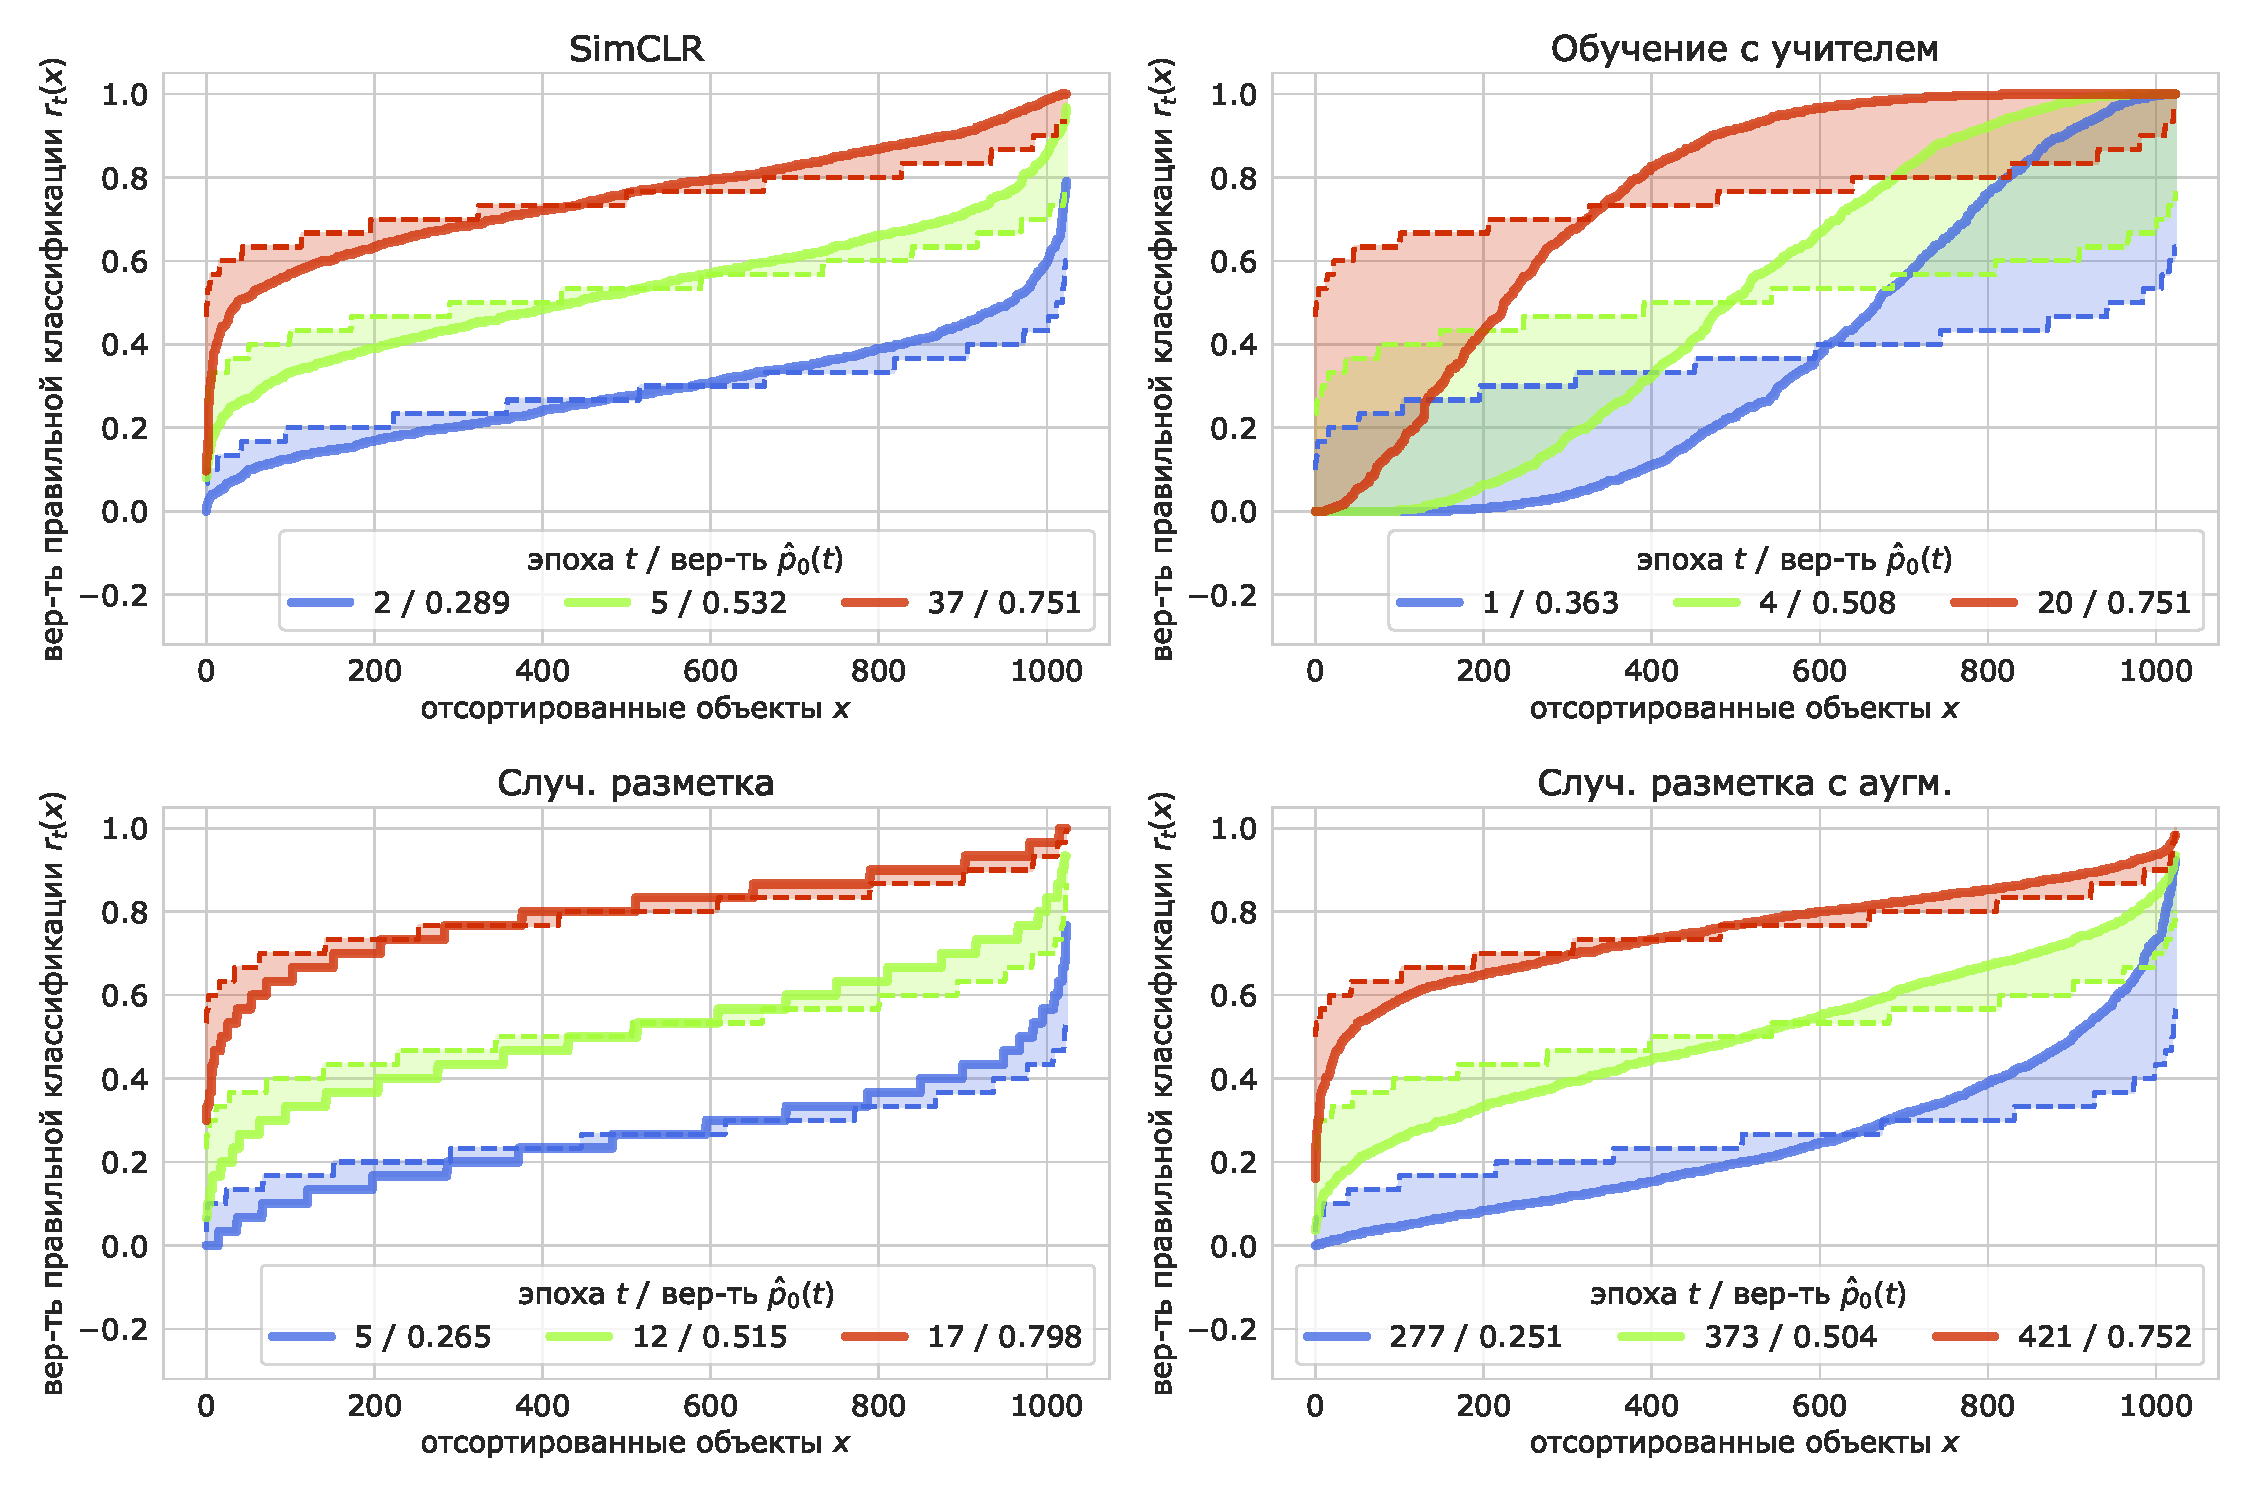
\includegraphics[width=17cm]{images/binom_noise2.pdf}
    \caption{Сравнение величины $r_t(x)$ (сплошная жирная линия) с соответствующим биномиальным шумом (пунктирная линия).}
    \label{experiments:pic:4}
\end{figure}{}

На рис. \ref{experiments:pic:4} и в таблице \ref{experiments:table:2} показаны результаты сравнения величины $r_t(x)$ с биномиальным шумом. Данный эксперимент подтверждает, что метод SimCLR и обе вариации обучения со случайной разметкой имеют меньший разброс сложностей объектов, чем обучение с учителем. Сравнивая данную группу графиков с предыдущей, мы приходим к выводу, что усреднение по аугментациям выравнивает сложности объектов в методе SimCLR. Заключительный эксперимент текущей серии проверяет данную гипотезу.

\begin{table}[H]
    \centering
    \begin{tabular}{|C{2.5cm}|C{1.75cm}|C{2.75cm}|C{3.25cm}|}
        \hline
        Метод & Эпоха $t$ & Вер-ть $\widehat{p}_0(t)$ & МАЕ ($\mu \pm \sigma$) \\ \hline
        \multirow{3}{*}{SimCLR} & 2 & 0.289 & $0.042 \pm 0.001$ \\ \cline{2-4}
        & 5 & 0.532 & $0.055 \pm 0.002$ \\ \cline{2-4}
        & 37 & 0.751 & $0.048 \pm 0.001$ \\ \hline
        \multirow{3}{*}{\shortstack{Обучение \\ с учителем}} & 1 & 0.363 & $0.248 \pm 0.001$ \\ \cline{2-4}
        & 4 & 0.508 & $0.267 \pm 0.002$ \\ \cline{2-4}
        & 20 & 0.751 & $0.208 \pm 0.001$ \\ \hline
        \multirow{3}{*}{\shortstack{Случ. \\ разметка}} & 5 & 0.265 & $0.037 \pm 0.002$ \\ \cline{2-4}
        & 12 & 0.515 & $0.052 \pm 0.001$ \\ \cline{2-4}
        & 17 & 0.798 & $0.031 \pm 0.002$ \\ \hline
        \multirow{3}{*}{\shortstack{Случ. \\ разметка \\ с аугм.}} & 277 & 0.251 & $0.093 \pm 0.002$ \\ \cline{2-4}
        & 373 & 0.504 & $0.081 \pm 0.001$ \\ \cline{2-4}
        & 421 & 0.752 & $0.038 \pm 0.002$ \\ \hline
    \end{tabular}
    \caption{Результаты сравнения величины $r_t(x)$ с биномиальным шумом. Для каждого подсчета метрики MAE было сгенерировано по 10 выборок биномиального шума, в таблице представлены среднее значение и стандартное отклонение.}
    \label{experiments:table:2}
\end{table}

На рис. \ref{experiments:pic:5} показано, как именно распределена величина $\tilde{r}_t(\tilde{x})$ для каждого фиксированного объекта $x$ и его аугментаций $\tilde{x} \sim \mathcal{A}(\tilde{x}|x)$. Согласно графику, в методе SimCLR многие аугментированные версии изображений являются либо очень сложными, и почти никогда не классифицируются правильно, либо очень простыми, и почти всегда верно распознаются нейронной сетью. Тем не менее, сами объекты тоже обладают разной сложностью: некоторые из них в принципе не имеют простых (или сложных) аугментаций. Напротив, при обучении с учителем и со случайной разметкой сложность аугментаций отличается не сильно: точки для разных аугментаций расположены вблизи среднего значения.

Мы связываем данный эффект с тем, что метод SimCLR использует более интенсивные аугментации. Они необходимы, чтобы сделать задачу разбиения изображений на пары достаточно сложной. Решение подобной задачи заставляет нейронную сеть выделять семантические закономерности изображений, что будет показано в \hyperref[visual:1]{разделе 5.1}.

\begin{figure}[H]
    \centering
    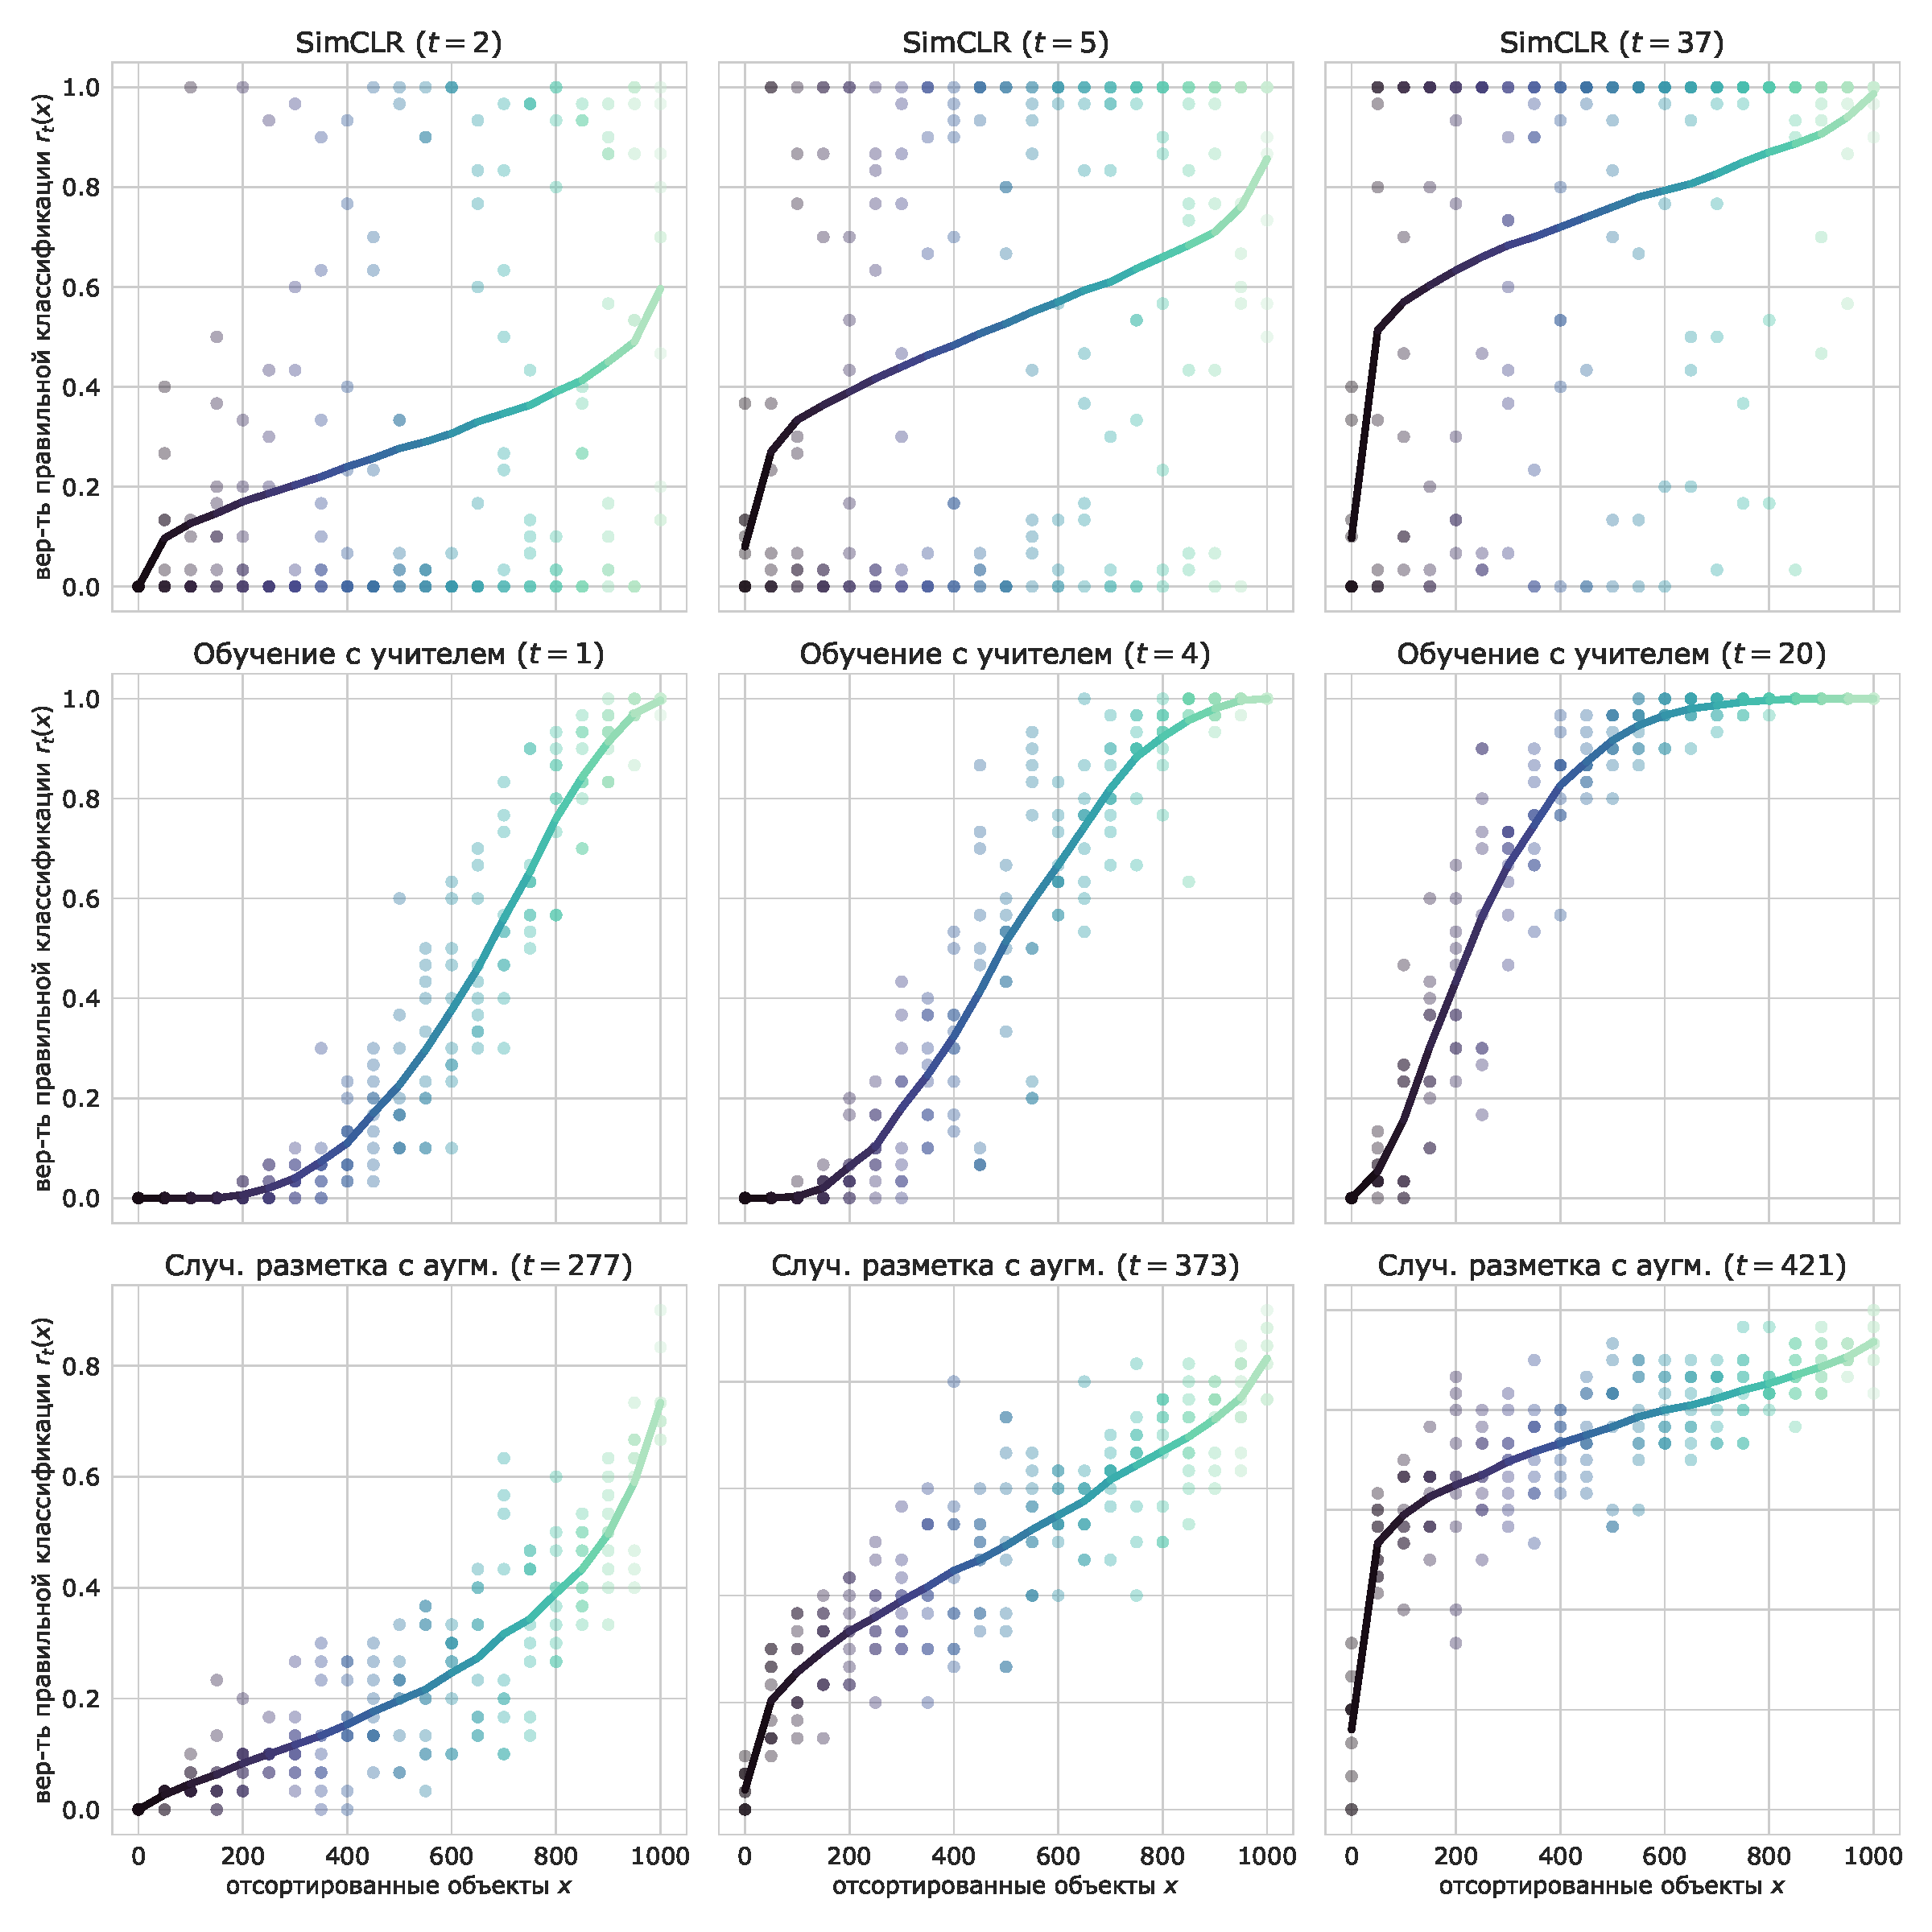
\includegraphics[width=17cm]{images/augments.pdf}
    \caption{Влияние аугментаций на сложности объектов для методов обучения. Каждая точка на графике --- значение $\tilde{r}_t(\tilde{x})$ для одной аугментации $\tilde{x}$. Для отображения был выбран каждый 50-ый объект среди отсортированной обучающей подвыборки. Сплошная кривая представляет собой усреднение по аугментациям, то есть величину $r_t(x)$.}
    \label{experiments:pic:5}
\end{figure}{}

Итак, эксперименты данного раздела демонстрируют, что для каждого алгоритма обучения существуют априорные сложности объектов: какие-то изображения распознаются нейронной сетью лучше и чаще классифицируются правильно; на других изображениях, напротив, нейронная сеть чаще ошибается. При этом описанный эффект в большей или меньшей степени проявляется для всех алгоритмов. Мы констатируем, что наибольший разброс сложности объектов наблюдается при обучении с учителем. Также мы показываем, что аугментации в методе SimCLR приводят к дополнительному ''расслоению'' сложностей: если зафиксировать по одной аугментации изображения, то разброс сложностей напоминает обучение с учителем. Однако усреднение по аугментациям выравнивает сложности объектов, и по данному показателю метод SimCLR становится похож на обучение со случайной разметкой.


\section{Визуализации}
\subsection{Визуализации представлений}
\label{visual:1}

Продолжая анализ, мы сравниваем векторные представления, которые получаются у нейронных сетей, обученных разными методами (здесь число эпох обучения методов следующее: $t=200$ для SimCLR, $t=200$ для обучения с учителем, $t=30$ для случайной разметки и $t=500$ для случайной разметки с аугментациями). Для этого у нейронных сетей отбрасывается последний линейный слой, после чего обучаются двумерные t-SNE представления (англ. t-distributed stochastic neighbor embedding) \cite{tsne} на выходах предпоследнего слоя для части обучающих объектов. Данные выходы имеют размерность $D=512$. Мы используем случайные 25\% обучающей выборки с сохранением баланса классов (для CIFAR-10 это $0.25 \cdot 50000 = 12500$ объектов).

На рис. \ref{visual:pic:1} изображены обученные t-SNE представления для четырех анализируемых постановок. Метод SimCLR заметно отличается от алгоритмов классификации разметки (истинной или случайной): представления последних образуют четкие кластеры, которые выделяются методом t-SNE. Данные кластеры должны быть линейно разделимыми, чтобы последний линейный слой мог правильно их классифицировать. Разумеется, кластеры согласуются с истинной разметкой только в случае обучения с учителем. При этом добавление аугменаций к обучению со случайной разметкой делает расположение кластеров более плотным.

\begin{figure}[H]
    \centering
    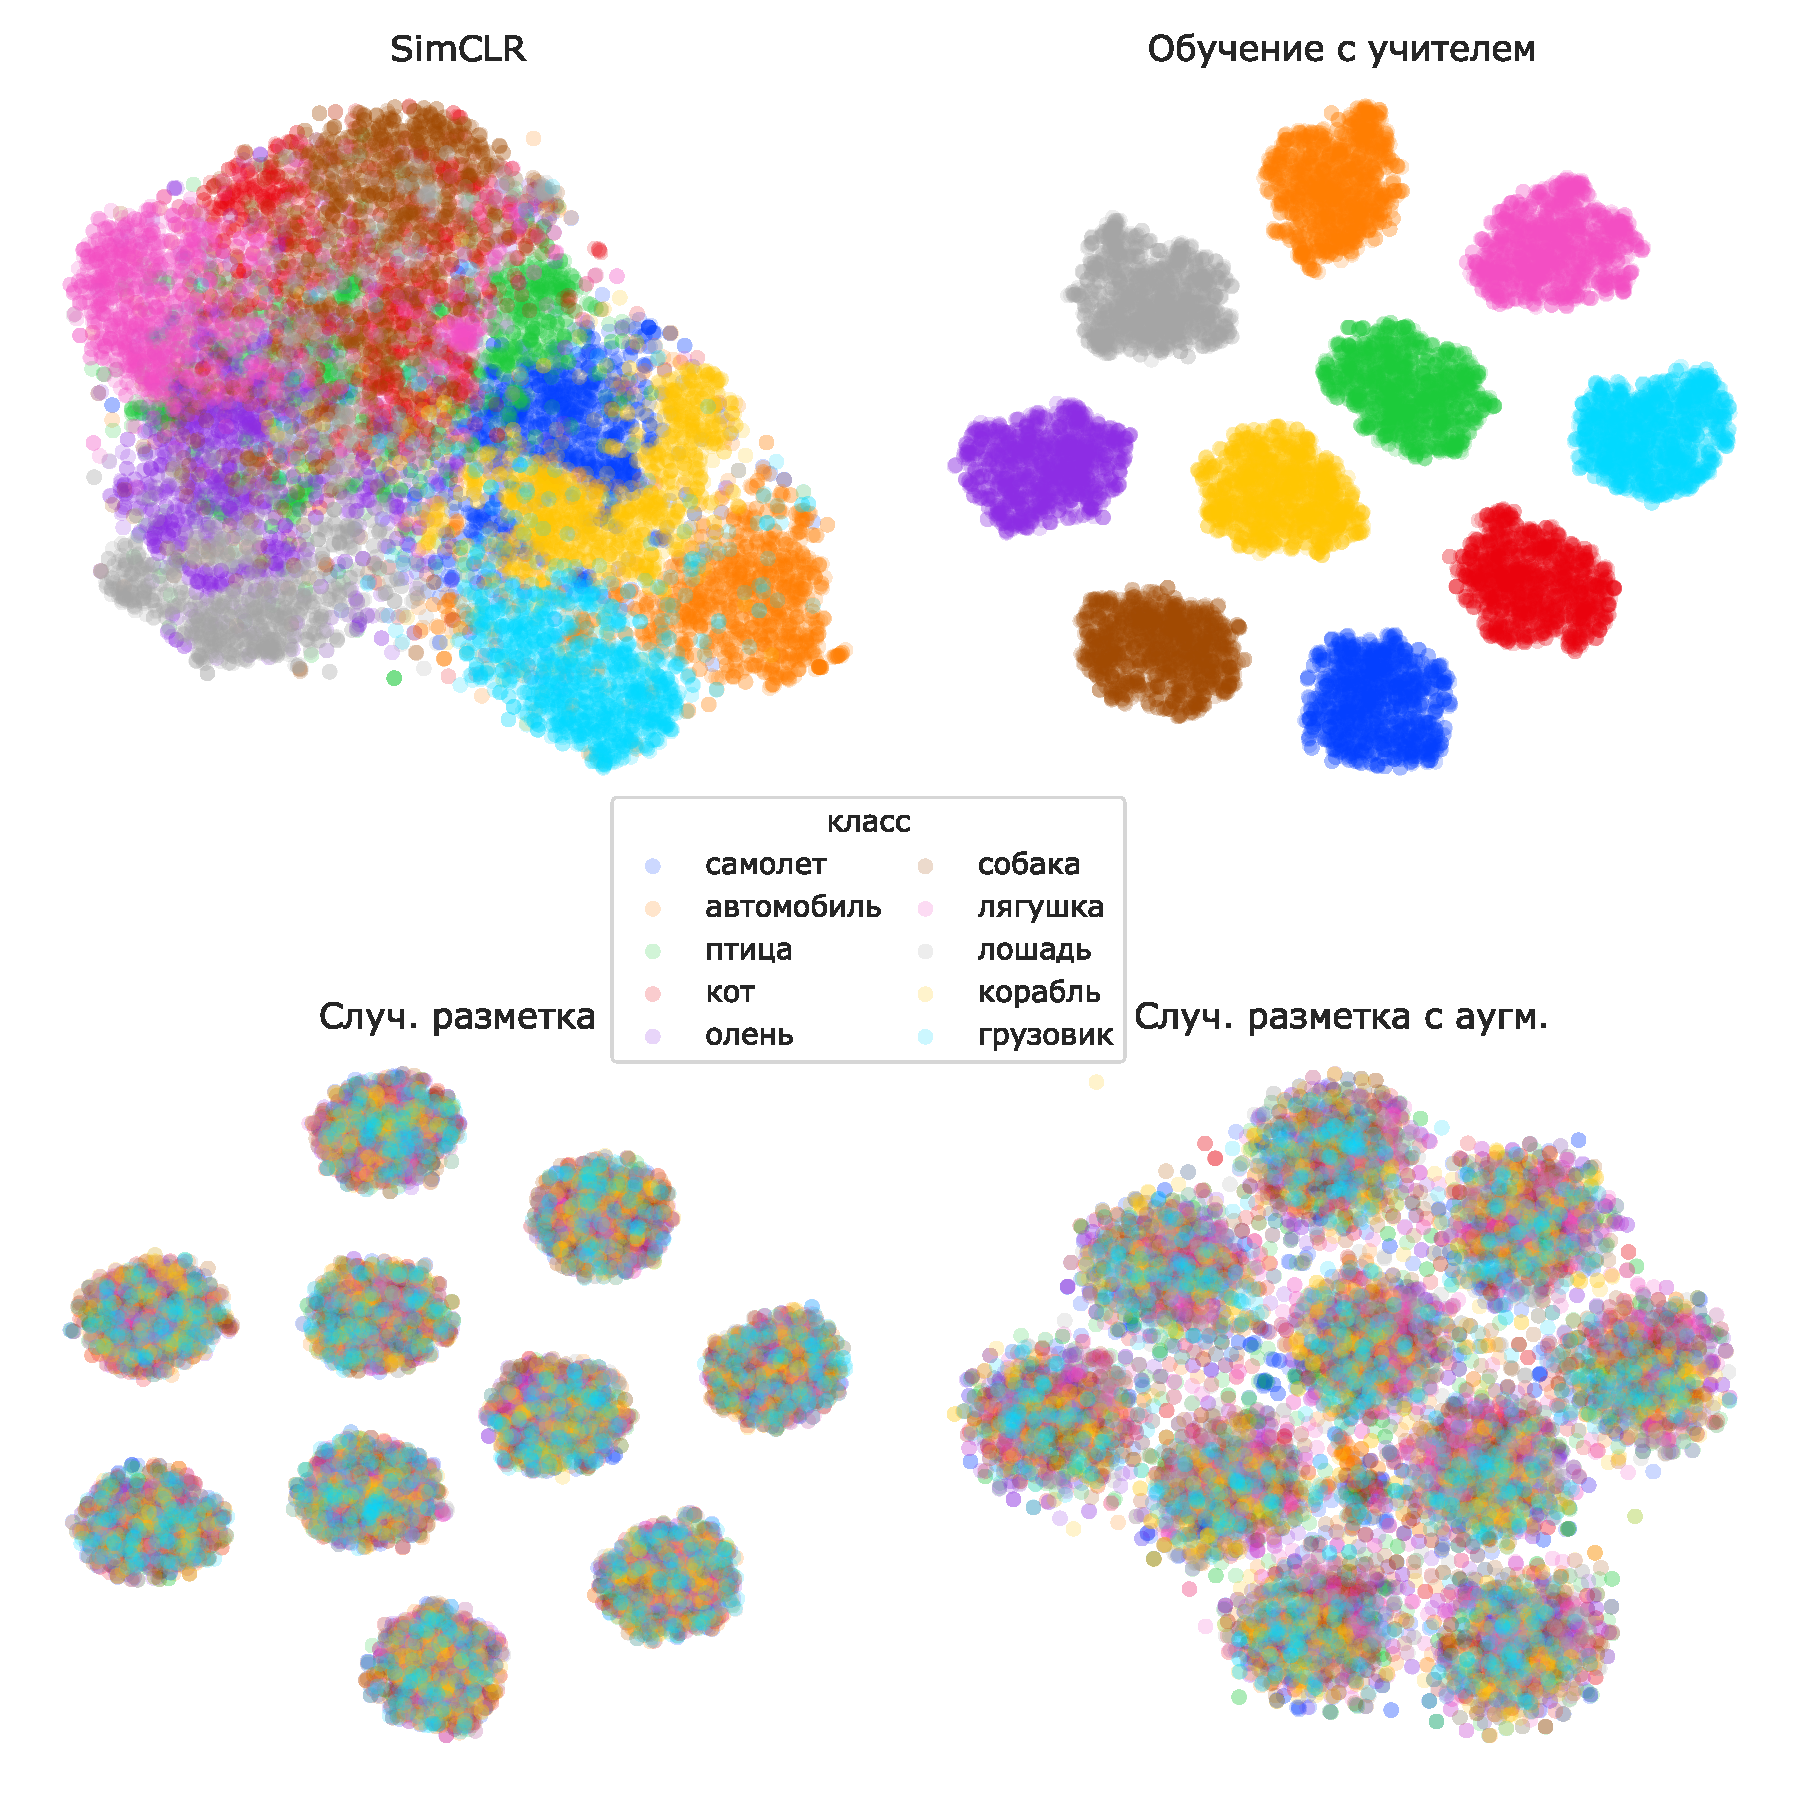
\includegraphics[width=17cm]{images/tsne.pdf}
    \caption{t-SNE представления выходов нейронных сетей, обученных разными методами, для 25\% обучающих объектов. Цветами показана принадлежность обучающих объектов к классам CIFAR-10.}
    \label{visual:pic:1}
\end{figure}{}

Однако наиболее плотное скопление t-SNE представлений наблюдается у алгоритма SimCLR. Это объясняется тем, что нейронная сеть при обучении методом SimCLR не получает сигналов на рассталкивание классов, как происходит при обучении с кросс-энтропийной функцией потерь. Минимизация последней связана не с правильной классификацией обучающих объектов, а с присвоением единичной вероятности истинному классу и нулевой вероятности остальным классам. Поэтому даже если выходы предпоследнего слоя оказываются линейно разделимы, то нейронная сеть продолжает отдалять друг от друга сложившиеся кластеры, повышая верояность истинного класса. В случае метода SimCLR такого эффекта нет, что приводит к более плотному расположению векторных представлений.

Тем не менее, из рис. \ref{visual:pic:1} видно, что t-SNE представления метода SimCLR относительно неплохо согласуются с истинной разметкой по классам. Мы проводим дополнительный эксперимент, сравнивающий взаимное расположение векторных представлений разных классов. Пусть $\{u_k^y\}_{k=1}^{K_y}$ --- это выходы предпоследнего слоя нейронной сети для обучающих объектов класса $y \in \{1, \dots, L\}$, где $L$ --- общее число классов и $u_k^y \in \R^D$. Приблизим распределение $u_k^y$ нормальным $\mathcal{N}_y(\mu_y, \Sigma_y)$ с параметрами:
\begin{equation}
    \mu_y = \frac{1}{K_y} \sum_{k=1}^{K_y} u_k^y \quad\quad \Sigma_y = \frac{1}{K_y - 1} \sum_{k=1}^{K_y} \big(u_k^y - \mu_y\big) \big(u_k^y - \mu_y\big)^T
\end{equation}

\noindent
Мы предлагаем считать KL-дивергенцию между нормальными распределениями, соответствующими разным классам, и сравнивать метод SimCLR и обучение с учителем по данному показателю. Пусть $y, z \in \{1, \dots, L\}$. Тогда KL-дивергенция между распределениями $\mathcal{N}_y(\mu_y, \Sigma_y)$ и $\mathcal{N}_z(\mu_z, \Sigma_z)$ вычисляется по формуле, выведенной в \cite{kl}:
\begin{equation}
\begin{aligned}
    \text{KL}\big(\mathcal{N}_y \big|\big| \mathcal{N}_z\big) = \frac{1}{2} \bigg(\text{Tr}\big(\Sigma_z^{-1} \Sigma_y\big) &+ \big(\mu_z - \mu_y\big)^T \Sigma_z^{-1} \big(\mu_z - \mu_y\big) + \\
    &+ \ln \frac{|\Sigma_z|}{|\Sigma_y|} - D\bigg)
\end{aligned}
\end{equation}

На рис. \ref{visual:pic:2} изображены значения KL-дивергенции, построенные описанным выше способом. Данный эксперимент подтверждает предыдущие выводы: при обучении с учителем векторные представления разных классов оказываются сильно разделены, в то время как SimCLR сохраняет плотную структуру представлений. При этом для метода SimCLR верно, что семантически похожие классы располагаются ближе, чем непохожие: например, дивергенция между классами ''кот'' и ''собака'' заметно меньше, чем между классами ''кот'' и ''автомобиль'' или ''собака'' и ''автомобиль''. Подобное наблюдение можно сделать и для обучения с учителем, но здесь значения KL-дивергенции отличаются в меньшее число раз. Таким образом, векторные представления, которые получаются у метода SimCLR, имеют определенную семантическую структуру, несмотря на то что при обучении не использовалась истинная разметка.

\begin{figure}[H]
    \centering
    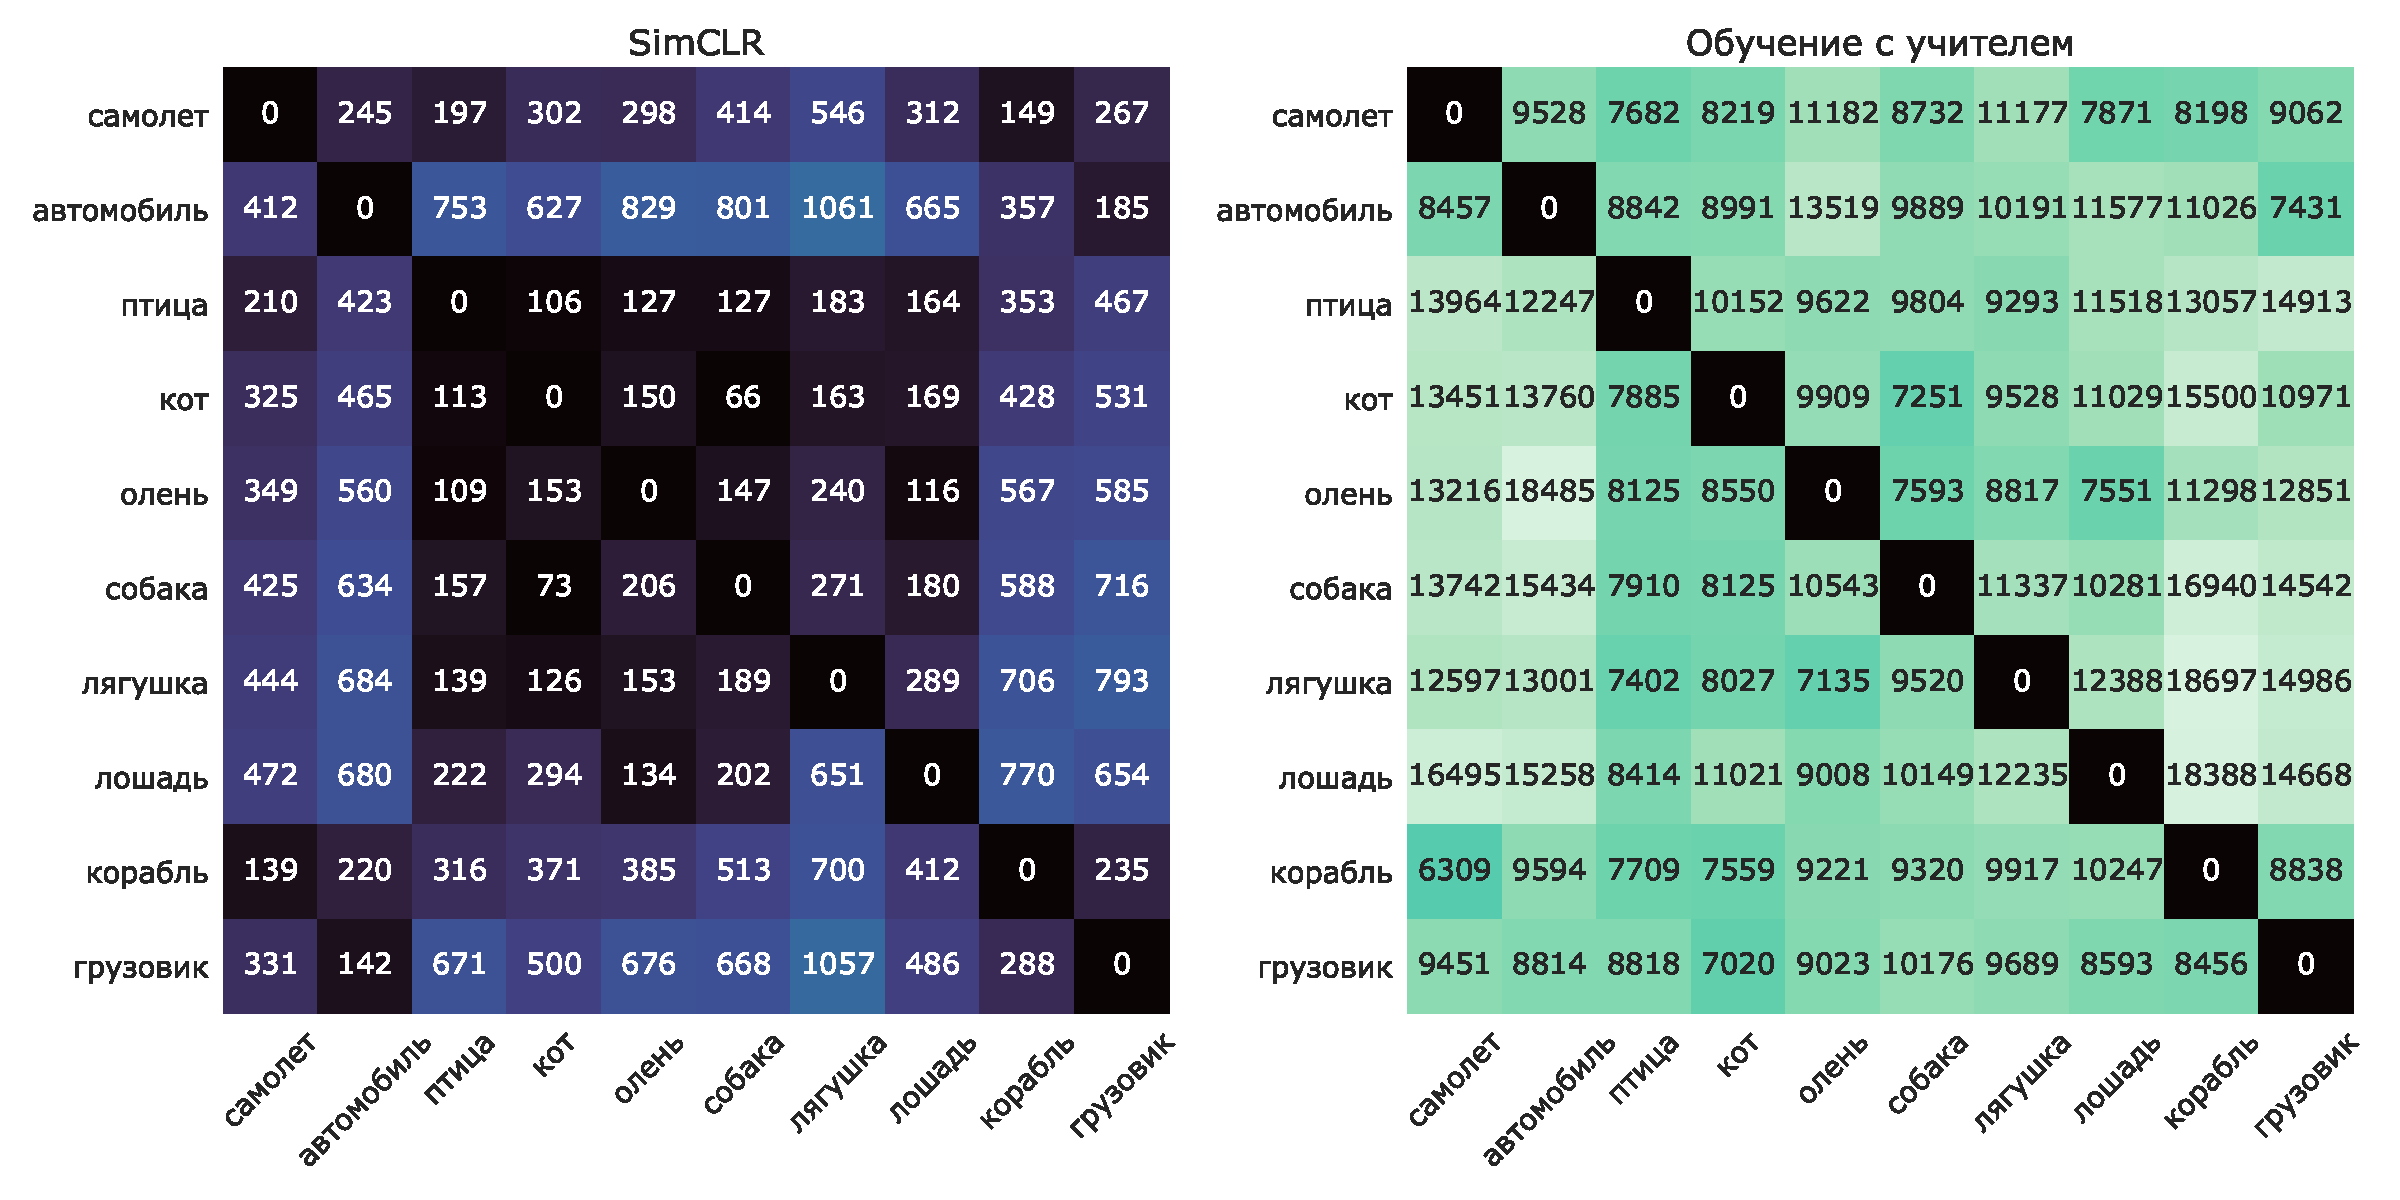
\includegraphics[width=17cm]{images/kl_divergence.pdf}
    \caption{Значения KL-дивергенции между нормальными распределениями, приближающими векторные представления объектов одного класса. Темные цвета соответствуют меньшим значениям дивергенции, светлые --- большим.}
    \label{visual:pic:2}
\end{figure}{}

Мы дополнительно анализируем, являются ли объекты разных классов сложными для выучивания при обучении нейронных сетей. Пусть $\mathcal{D}_y$ означает распределение изображений обучающей выборки, принадлежащих классу $y$. Мы оцениваем величину $\E_{x \sim \mathcal{D}_y} \big[r_t(x)\big]$ методом Монте-Карло:
\begin{equation}
    \E_{x \sim \mathcal{D}_y} \big[r_t(x)\big] \approx \frac{1}{K_y} \sum_{k=1}^{K_y} r_t(x_k^y),
\end{equation}

\noindent
где $\{x_k^y\}_{k=1}^{K_y}$ --- обучающая подвыборка изображений класса $y$. На рис. \ref{visual:pic:3} показана динамика данной величины при обучении методом SimCLR и при обучении с учителем. Из графиков видно, что в задаче классификации выделяются простые (''автомобиль'', ''грузовик'', ''корабль'') и сложные (''кот'', ''птица'', ''собака'') классы, которые выучиваются нейронной сетью, соответственно, быстрее и медленнее. В случае метода SimCLR, напротив, динамика между классами отличается не сильно. В \hyperref[experiments:1]{разделе} 4.2 было показано, что объекты при обучении с учителем значительно отличаются по сложности, и из данного графика следует, что принадлежность изображений разным классам является одной из причин наблюдаемого эффекта.

\begin{figure}[H]
    \centering
    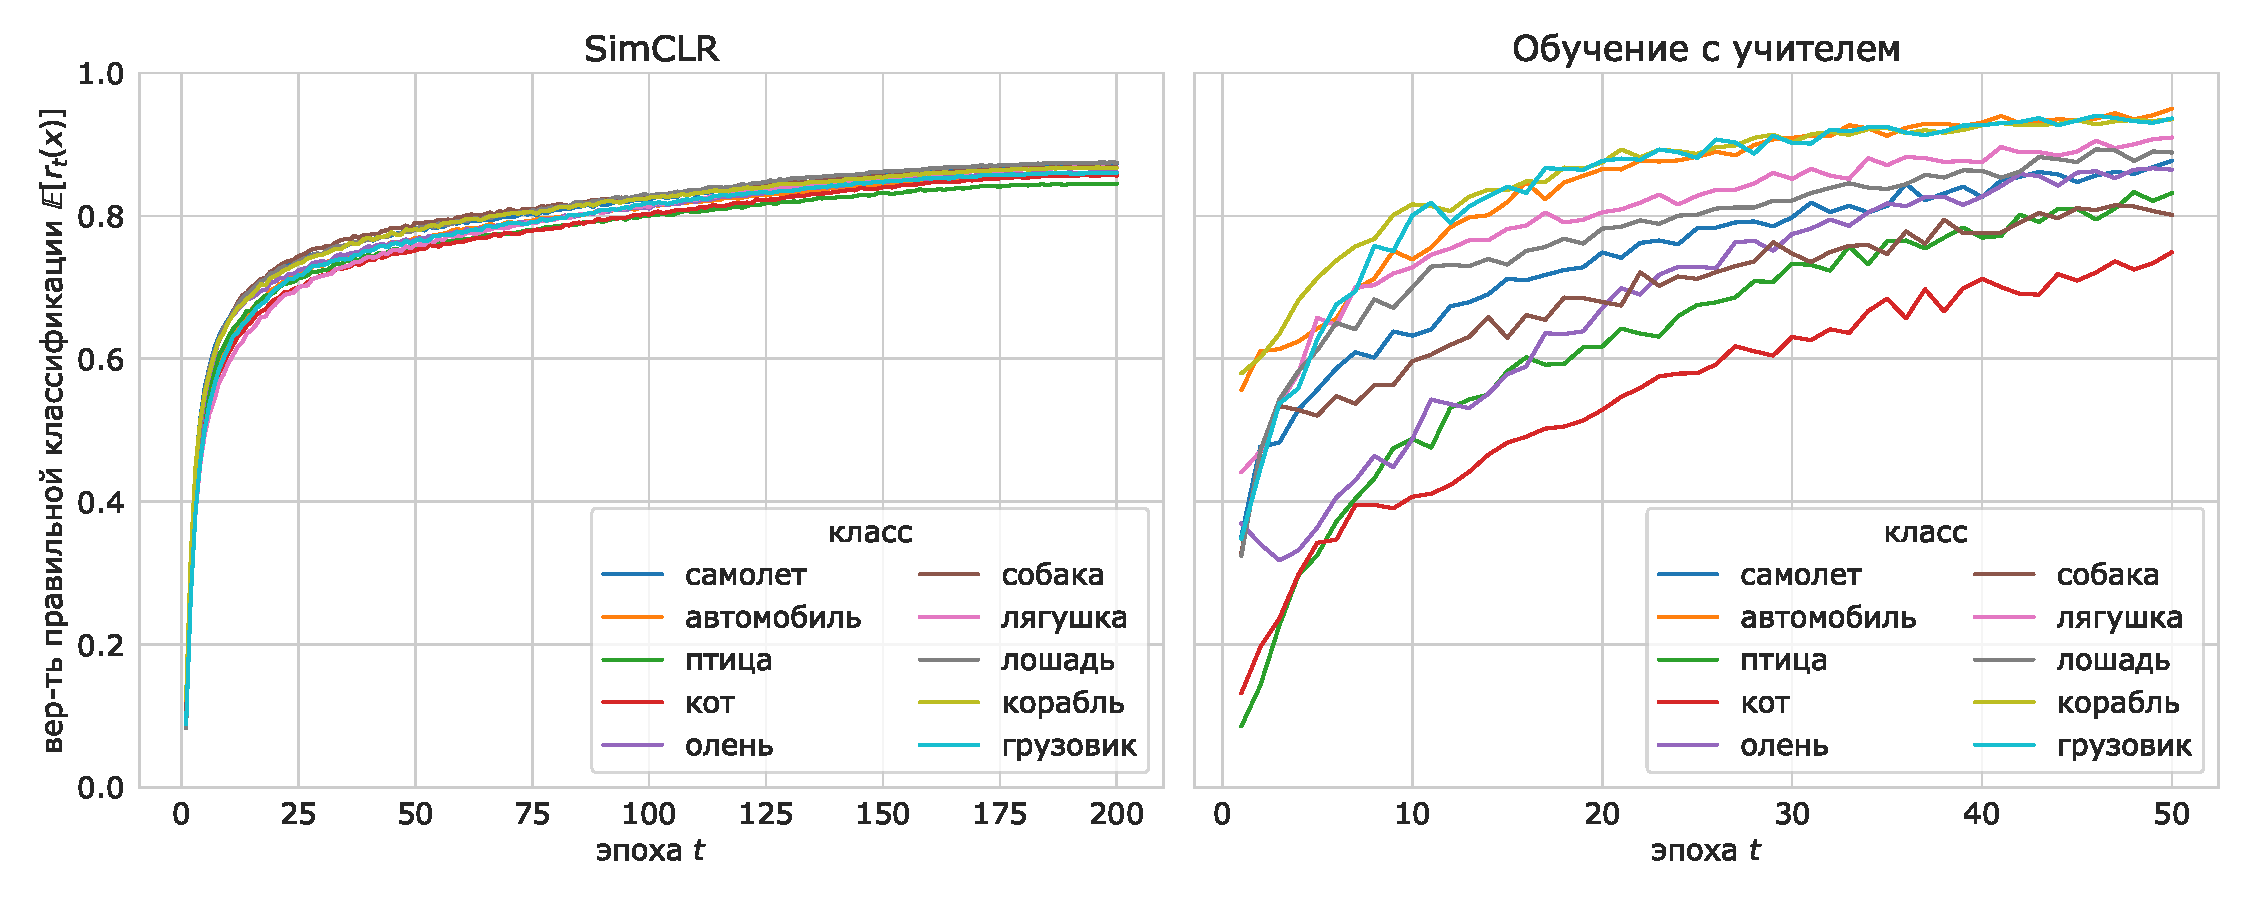
\includegraphics[width=17cm]{images/class_difficulties.pdf}
    \caption{Динамика величины $\E_{x \sim \mathcal{D}_y} \big[r_t(x)\big]$ по эпохам обучения $t$ для разных классов CIFAR-10.}
    \label{visual:pic:3}
\end{figure}{}

\subsection{Визуализации активаций}

В данной работе мы рассматриваем один из самых популярных подходов к визуализации обученных сверточных нейронный сетей --- визуализация рецептивного поля активаций с помощью градиентного подъема в пространстве пикселей \cite{visual}. Рассмотрим некоторую подсеть нейронной сети \linebreak $h: \R^{H_0 \times W_0 \times C} \rightarrow \R$, соответствующую одной активации (одному каналу карты признаков). $H_0 \times W_0$ --- размер рецептивного поля данной активации по отношению ко входу нейронной сети. Пусть тензор $x \in \R^{H_0 \times W_0 \times C}$, максимизурует активацию $h(x)$. Мы будем называть его \textit{псевдоизображением}. Задача оптимизации $h(x)$ по $x$ решается методом градиентного подъема с длиной шага $\eta=1$ и числом итераций $T=1000$. 

\begin{figure}[H]
    \centering
    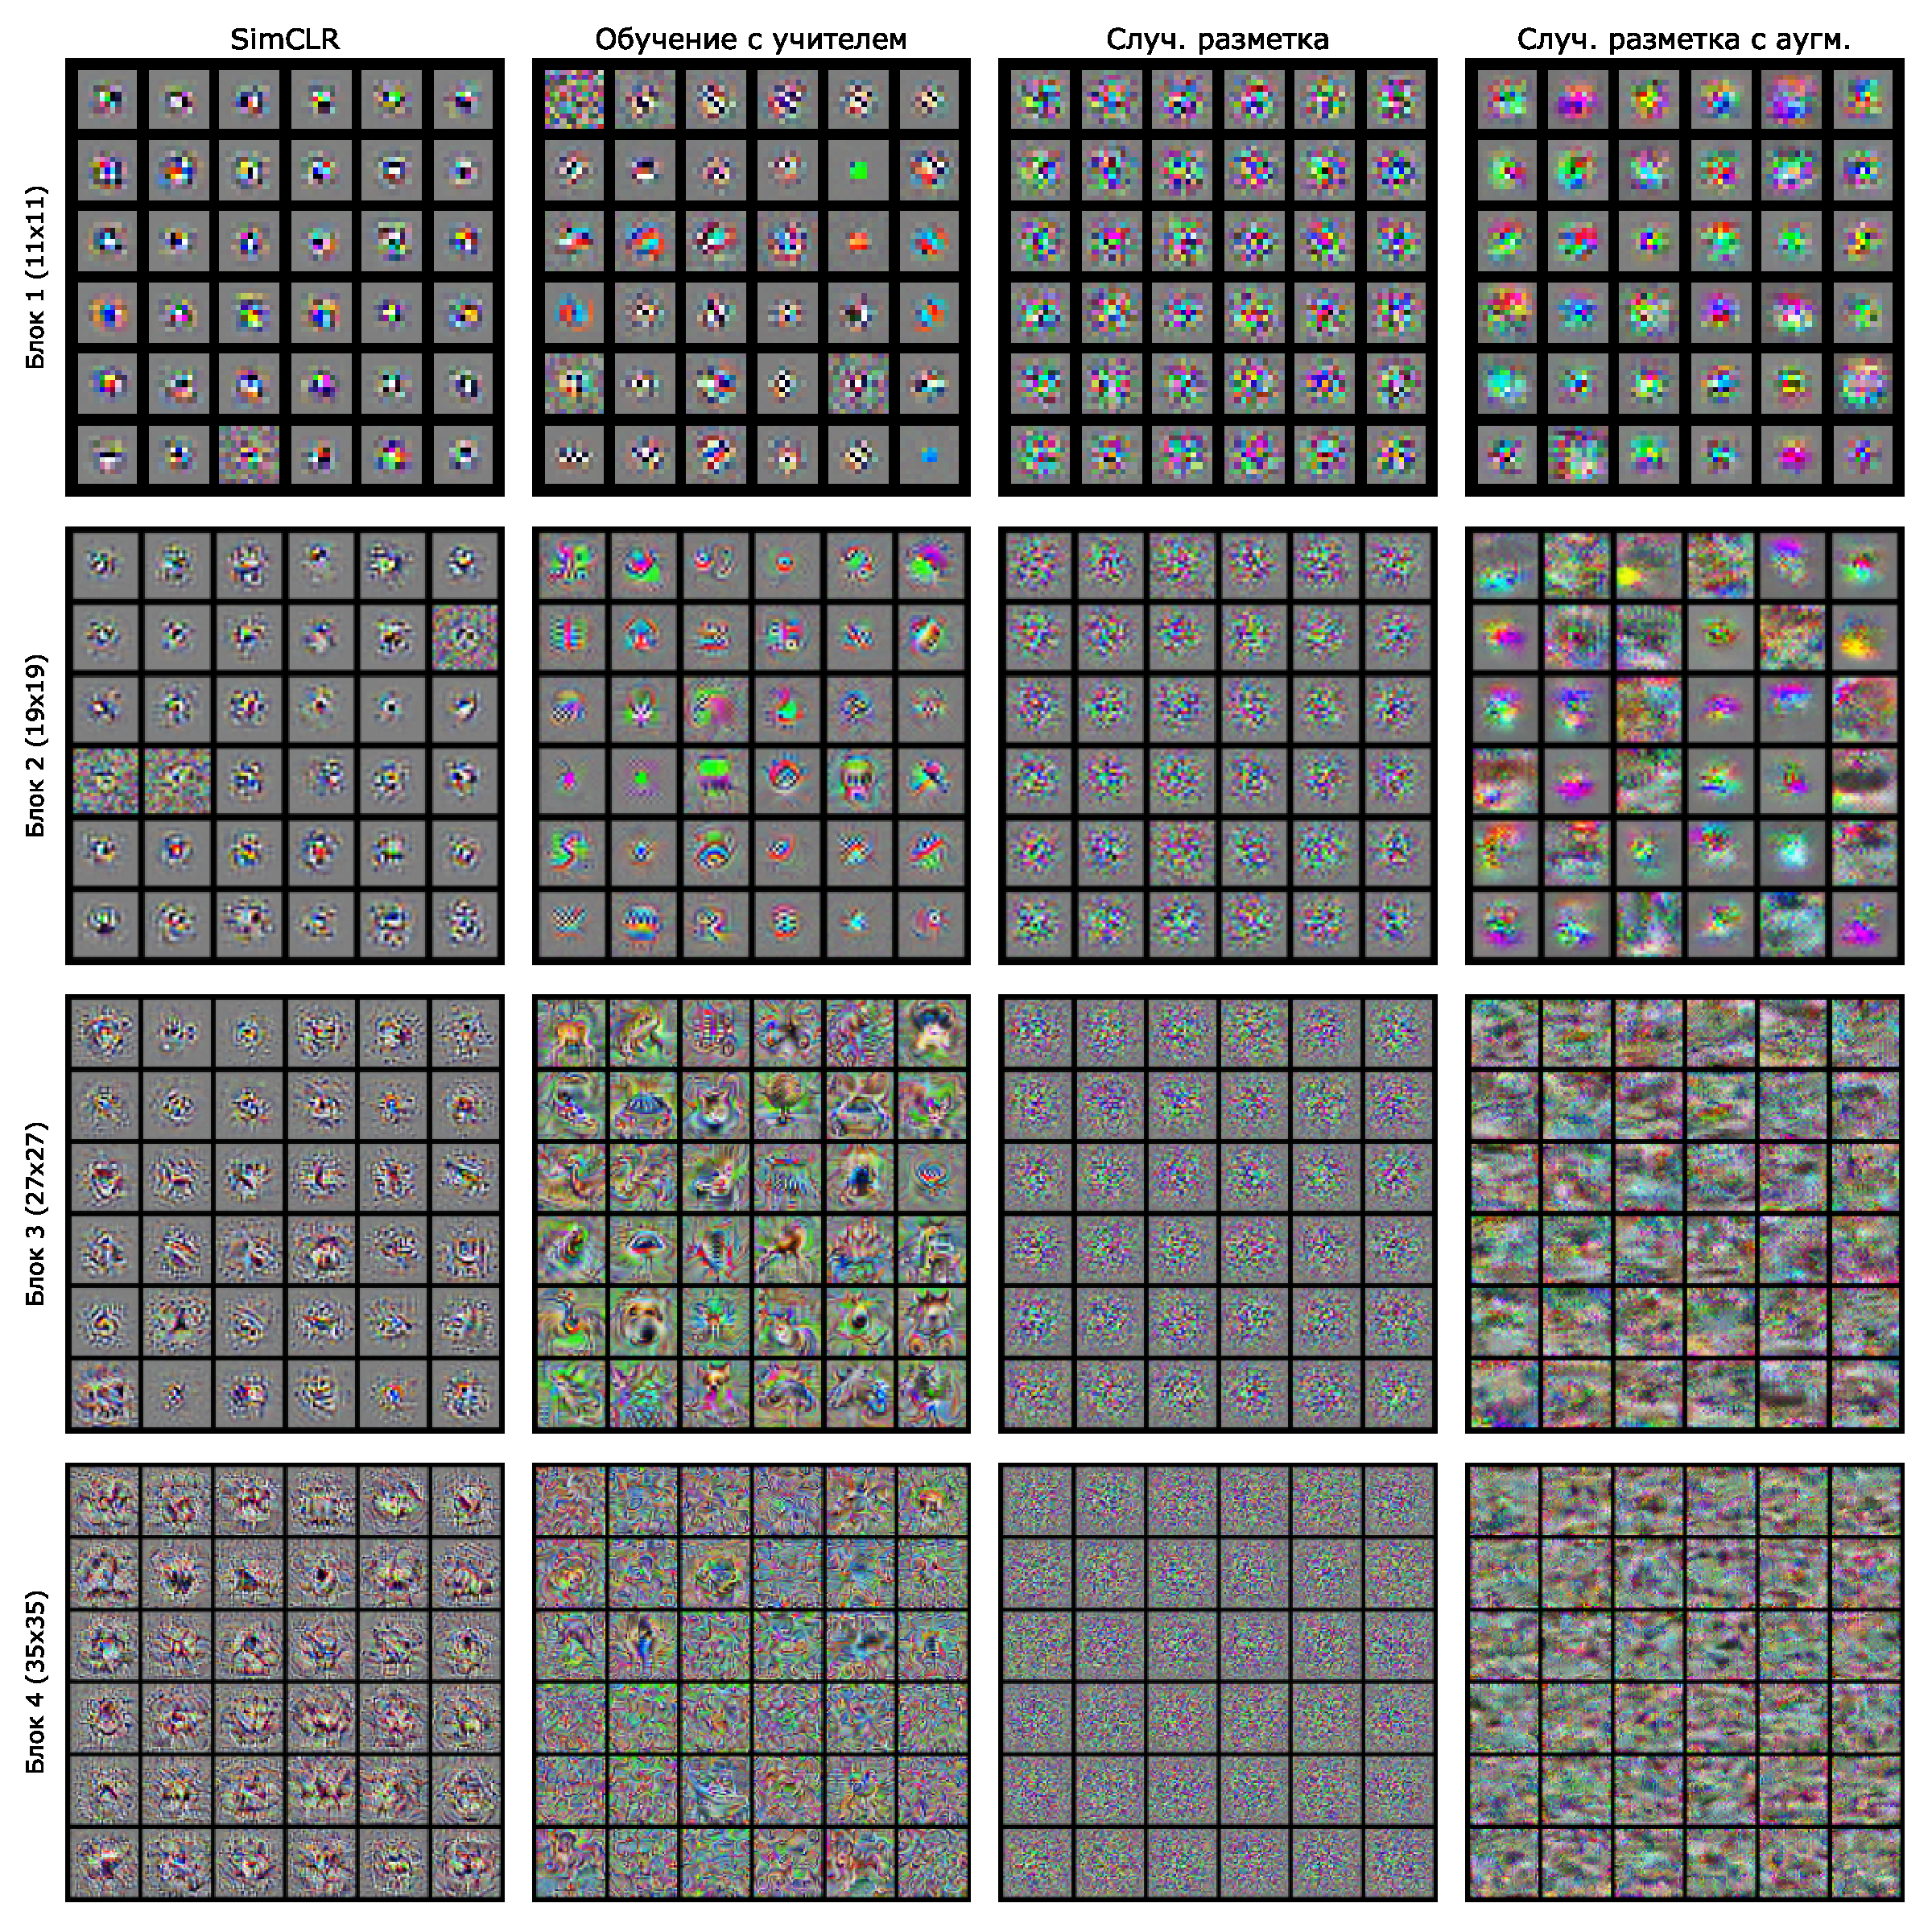
\includegraphics[width=17cm]{images/activations.pdf}
    \caption{Визуализации активаций различных методов. Каждый столбец соответствует своему методу, каждый ряд --- активациям с выхода одного и того же блока архитектуры ResNet-18. В скобках указан размер рецептивного поля активаций $H_0 \times W_0$. Каналы карт признаков для визуализации выбирались случайно, по 36 на каждую пару (метод, блок).}
    \label{visual:pic:4}
\end{figure}{}

Отдельно стоит отметить метод нормализации, который применялся для рисования полученных псевдоизображений. Дело в том, что тензоры, полученные при решении оптимизационной задачи, могут содержать произвольные вещественные числа, в то время как пиксели цветого пространства RGB ограничены отрезком $[0, 1]$. Для каждого псевдоизображения $x$ мы получаем его нормализацию $\hat{x}$ по следующей формуле:
\begin{equation}
\begin{gathered}
    \hat{x} = \sigma \left(\frac{x - \mu_{x}}{s_x}\right)\text{, где} \\
    \mu_x = \frac{1}{H_0 \cdot W_0 \cdot C} \sum_{h, w, c} x_{h, w, c} \quad\quad
    s_x = \sqrt{\frac{1}{H_0 \cdot W_0 \cdot C- 1} \sum_{h, w, c} (x_{h, w, c} - \mu_x)^2}
\end{gathered}
\end{equation}

\noindent
Здесь $\sigma(t)=1/(1+\exp(-t))$ --- логистическая функция, необходимая для отображения значений в отрезок $[0, 1]$.

На рис. \ref{visual:pic:4} показаны визуализации активаций с различных слоев нейронной сети для четырех алгоритмов обучения. Использовался описанный выше метод нормализации псевдоизображений. Сильнее всего выделяются визуализации для обучения со случайной разметкой, которые являются плохо интерпретируемым случайным шумом. Добавление аугментаций в обучение со случайной разметкой значительно меняет активации нейронной сети. Несмотря на то, что на визуализациях не прослеживаются характерные черты изображений CIFAR-10, псевдоизображения куда меньше напоминают шум. Визуализации для обучения с учителем и метода SimCLR похожи друг на друга: простые узоры на ранних слоях (блоки 1--2) переходят в более сложные орнаменты на поздних слоях (блоки 3--4). При этом визуализации метода SimCLR представляются более абстрактными и менее интерпретируемыми. В то же время, среди псевдоизображений обучения с учителем прослеживаются черты, характерные для классов CIFAR-10 (например, силуэт лошадиной \linebreak головы --- блок 3, второй ряд снизу, крайний правый столбец). Последнее наблюдение подтверждает интуицию, что при обучении с учителем нейронная сеть выделяет на обучающих изображениях фрагменты, характерные для классов разметки, и выдает предсказания, основываясь на соответствии входного изображения выделенным фрагментам.


\section{Заключение}
В данной работе мы проводим сравнительный анализ нескольких постановок обучения нейронных сетей: обучения в парадигме self-supervised learning на примере алгоритма SimCLR, обучения с учителем на классификацию изображений и обучения со случайной разметкой по классам. Мы изучаем динамику обучения и сложность объектов с точки зрения выучивания их нейронными сетями. Мы показываем, что в контексте всех постановок обучающие объекты имеют неодинаковую сложность. Наряду с этим, обучению с учителем свойственнен наибольший разброс сложности объектов. При фиксированных аугментациях изображений сложности объектов в методе SimCLR напоминают обучение с учителем, однако усреднение по аугментациям выравнивает сложности, что позволяет соотнести данный метод и обучение со случайной разметкой.

Мы приводим эмпирическое подтверждение того, что две указанные постановки имеют схожую динамику обучения. Мы объясняем данный феномен тем, что нейронные сети и в методе SimCLR, и при обучении со случайной разметкой должны научиться распозавать обучающие объекты. Данное предположение отличает указанные постановки от обучения с учителем, где для правильной классификации нейронной сети достаточно выделить фрагменты изображений, специфичные для каждого класса. Тем не менее, наш анализ обученных векторных представлений показывает, что представления метода SimCLR имеют четкую семантическую структуру, в отличие от представлений обучения со случайной разметкой. Данное наблюдение устанавливает связь между обучением с учителем и методом SimCLR, несмотря на то что при обучении последнего не используется разметка по классам изображений.

В заключение можно сказать, что динамика нейронных сетей, обученных в парадигме self-supervised learning, похожа на динамику обучения со случайной разметкой, однако поскольку нейронные сети обучаются не на случайный шум, а на некоторую содержательную задачу, то предобучение таким способом является полезным для использования нейронных сетей на других задачах компьютерного зрения.


\newpage
\section*{Список литературы} 
\addcontentsline{toc}{section}{Список литературы}
\printbibliography[heading=none]

\newpage
\section*{Приложения}
\addcontentsline{toc}{section}{Приложения}

\subsection*{Приложение А. Гиперпараметры обучения методов.} 
\addcontentsline{toc}{subsection}{Приложение А. Гиперпараметры обучения методов.}
\label{appendix:1}

Эксперименты проводились с использованием библиотеки PyTorch \cite{pytorch} языка программирования Python 3. Применялся сторонний репозиторий с кодом, содержащий реализацию метода SimCLR \cite{simclrrepo}.

Обучение метода SimCLR велось с помощью оптимизатора Adam \cite{adam} с начальной длиной шага (англ. learning rate) $\eta=3\cdot 10^{-4}$ и коэффициентом убывания весов (англ. weight decay) $wd=10^{-4}$. При этом использовался косинусный отжиг длины шага \cite{cosine}. Другие гиперпараметры равнялись следующим значениям: размер пакета $B=256$, температура $\tau=0.07$, размерность выходного пространства $d=128$, максимальное число эпох обучения $t_{\max}=200$.

Для обучения с учителем и со случайной разметкой применялся стохастический градиентный спуск с параметром импульса $m=0.9$. Все остальные гиперпараметры обучения совпадали с методом SimCLR, кроме температуры $\tau=1$, размерности выходного пространства $d=10$ (число классов CIFAR-10) и максимального числа эпох обучения ($t_{\max}=50$ для обучения с учителем, $t_{\max}=20$ для случайной разметки и $t_{\max}=500$ для случайной разметки с аугментациями).

При обучении метода SimCLR использовались следующие аугментации:
\begin{itemize}
    \setlength\itemsep{-0.25em}
    \item вырезание случайного фрагмента изображения
    \item случайное отражение изображения по горизонтали
    \item случайное изменение яркости, контраста, насыщенности и оттенка
    \item случайная конвертация в черно-белое изображение
    \item гауссово размытие
\end{itemize}

\noindent
В случае обучения с учителем и обучения со случайной разметкой из указанных аугментаций применялось только вырезание случайного фрагмента изображения, а также поканальная нормализация изображений с вектором средних $\mu=(0.4914, 0.4822, 0.4465)$ и вектором стандартных отклонений $\sigma=(0.2023, 0.1994, 0.2010)$, характерными для набора данных CIFAR-10. На рис. \ref{appendix:pic:1} приведен фрагмент кода, уточняющий параметры использованных аугментаций.

\begin{figure}[H]
    \centering
    \renewcommand{\thefigure}{А.1}
    \setstretch{1.1}
    \begin{subfigure}[b]{0.8\textwidth}
        \centering
        \begin{lstlisting}[language=Python]
        import torchvision.transforms as T
        
        def get_simclr_transform(size):
            color_jitter = T.ColorJitter(brightness=0.8, contrast=0.8,
                                         saturation=0.8, hue=0.2)
            
            transform = T.Compose([
                T.RandomResizedCrop(size=size),
                T.RandomHorizontalFlip(),
                T.RandomApply([color_jitter], p=0.8),
                T.RandomGrayscale(p=0.2),
                T.GaussianBlur(kernel_size=int(0.1 * size)),
                T.ToTensor()
            ])
            
            return transform
        \end{lstlisting}
    \end{subfigure}
    \begin{subfigure}[b]{0.8\textwidth}
        \centering
        \begin{lstlisting}[language=Python]
        import torchvision.transforms as T
        
        def get_supervised_transform(size):
            transform = T.Compose([
                T.RandomCrop(size, padding=4),
                T.RandomHorizontalFlip(),
                T.ToTensor(),
                T.Normalize(mean=(0.4914, 0.4822, 0.4465),
                            std=(0.2023, 0.1994, 0.2010))
            ])
            
            return transform
        \end{lstlisting}
    \end{subfigure}
    \caption{Фрагмент кода на библиотеке PyTorch языка программирования Python 3, который генерирует аугментации для метода SimCLR (сверху) и для обучения с учителем (снизу).}
    \label{appendix:pic:1}
\end{figure}{}

\subsection*{Приложение Б. Дополнительные материалы экспериментов.} 
\addcontentsline{toc}{subsection}{Приложение Б. Дополнительные материалы экспериментов.}
\label{appendix:2}

Дополнительный проведенный эксперимент проверяет, что две аугментированные версии изображения в методе SimCLR имеют сопоставимые величины $r_t(x)$. Согласно рис. \ref{appendix:pic:2}, даже при рассмотрении одной пары аугментаций вероятности правильной классификации первой и второй версии изображения неплохо соотносятся, однако для некоторых изображений данные вероятности отличаются значительно. Усреднение по аугментациям нивелирует подобные объекты, уменьшая разницу в величине $r_t(x)$ между первыми и вторыми версиями изображений.

\begin{figure}[H]
    \centering
    \renewcommand{\thefigure}{Б.1}
    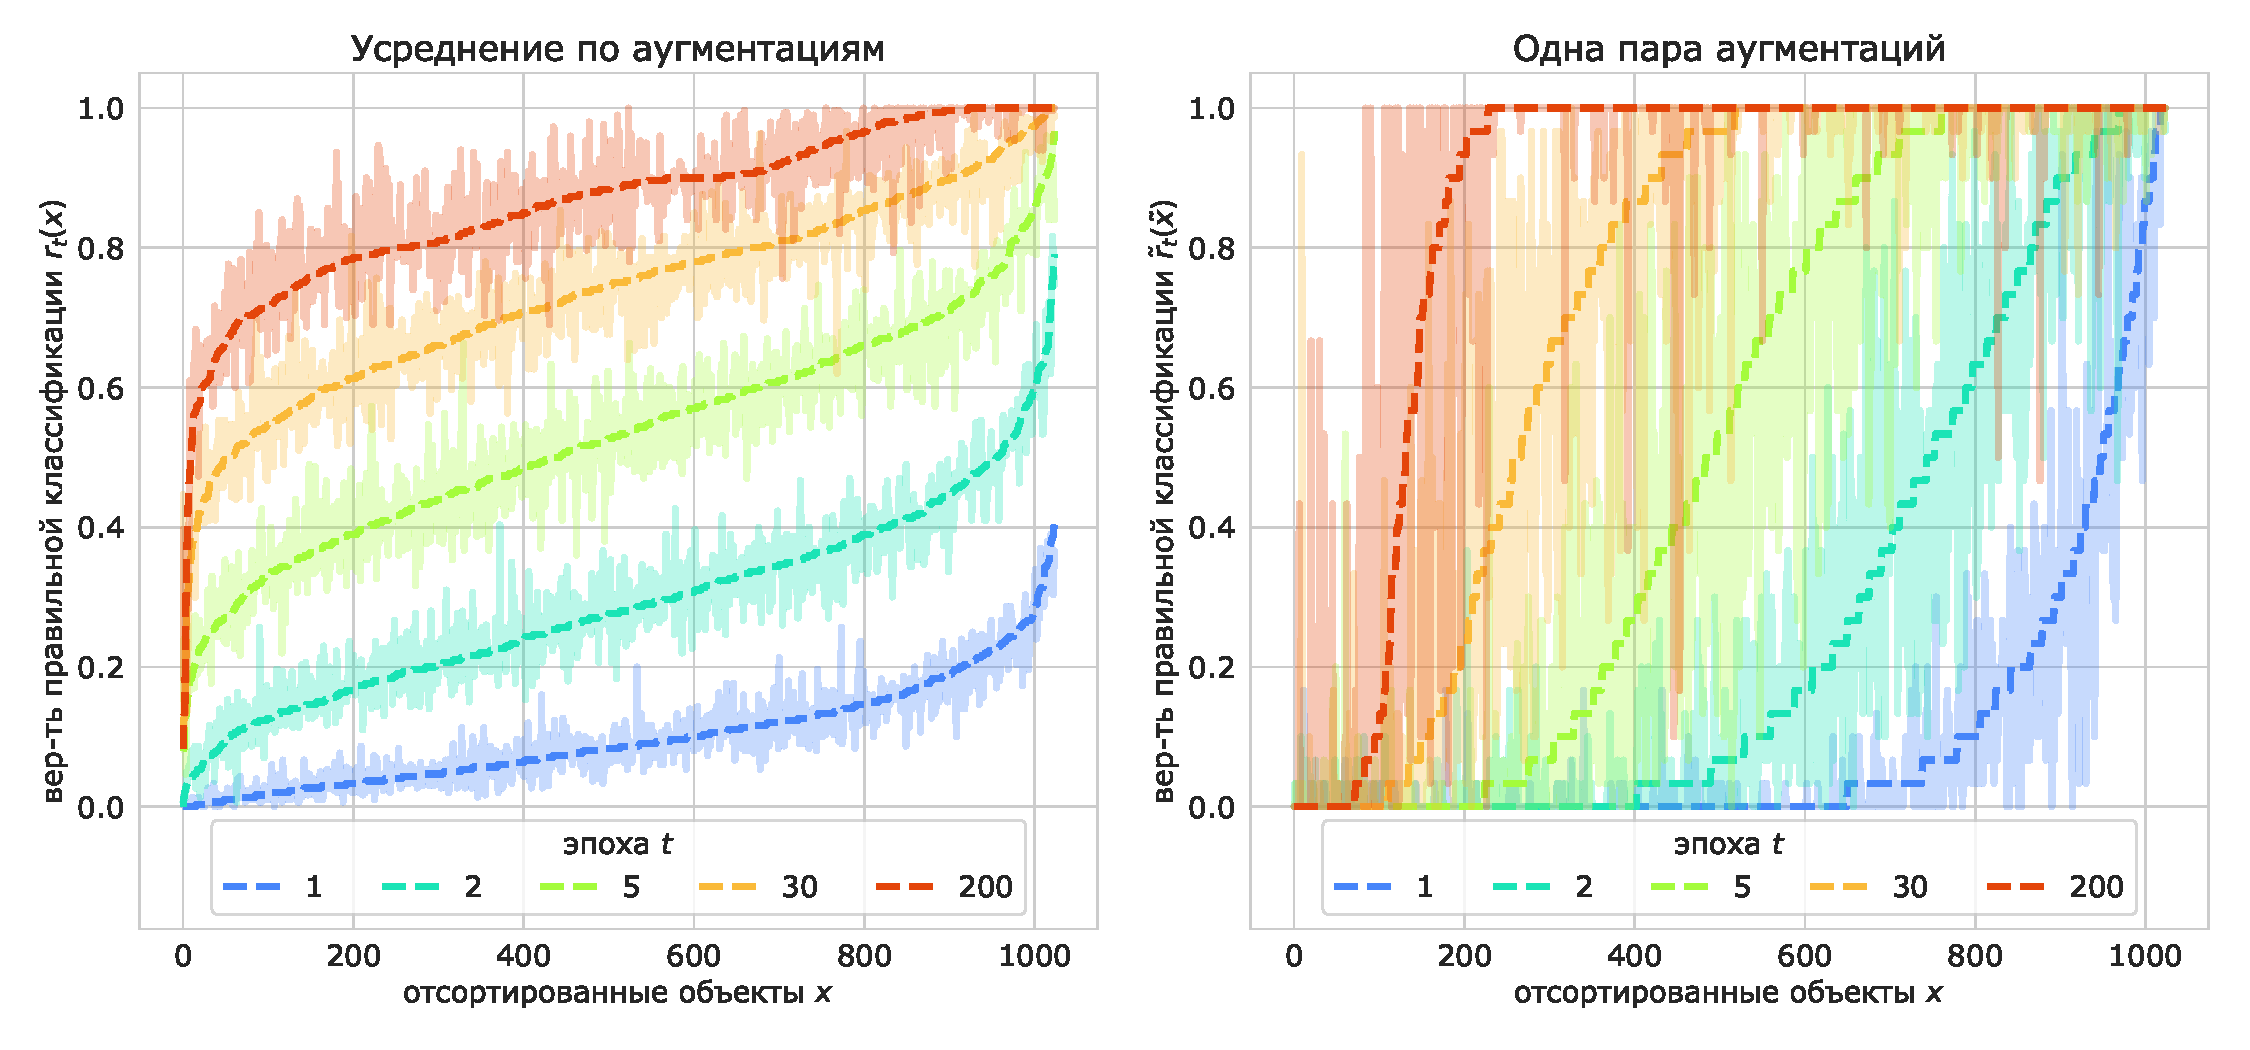
\includegraphics[width=17cm]{images/first_second.pdf}
    \caption{Сравнение величины $r_t(x)$ метода SimCLR, посчитанной по первым аугментациям изображений (пунктирная линия) и по вторым аугментациям изображений (полупрозрачная жирная линия), сортировка производится по величинам от первых аугментаций. Левый график соответствует величине $r_t(x)$, усредненной по аугментациям, а правый --- величине $\tilde{r}_t(\tilde{x})$, посчитанной по одной паре аугментаций.}
    \label{appendix:pic:2}
\end{figure}{}

Мы также проводим эксперимент, который сравнивает методы по качеству классификации на наборе данных CIFAR-10. Для этого у обученных нейронных сетей фиксируются веса, а поверх выходов предпоследнего слоя, имеющих разномерность $D=512$, обучается линейный классификатор (логистическая регресия без регуляризации). Используемый оптимизитор --- Adam с длиной шага $\eta=10^{-3}$, число эпох обучения $t=10$, размера пакета $B=256$. Помимо упомянутых в основной части методов, мы рассматриваем нейронную сеть со случайной инициализацией и обучение классификатора поверх исходных изображений. Результаты сравнения представлены в таблице \ref{appendix:tab:1}. 
\begin{table}[H]
    \centering
    \renewcommand{\thetable}{Б.1}
    \begin{tabular}{|C{5.25cm}|C{2.75cm}|C{2.75cm}|}
        \hline
         & Обучающая выборка & Тестовая выборка \\ \hline
        SimCLR \newline ($t=200$ эпох) & 0.8186	& 0.8060 \\ \hline
        Обучение с учителем \newline ($t=200$ эпох) & 1.0000 & 0.9532 \\ \hline
        Случ. разметка \newline ($t=30$ эпох) & 0.3369 & 0.3248 \\ \hline
        Случ. разметка с аугм. \newline ($t=500$ эпох) & 0.4395 & 0.4275\\ \hline
        Случ. \newline инциализация & 0.2891 & 0.2982\\ \hline
        Исходные \newline изображения & 0.4227 & 0.3768\\ \hline
    \end{tabular}
    \caption{Доля правильных ответов на наборе данных CIFAR-10 при обучении линейного классификатора поверх нейросетевых представлений.}
    \label{appendix:tab:1}
\end{table}

По доле правильных ответов закономерно выделяются обучение с учителем (как метод, который обучался непосредственно на классификацию CIFAR-10) и SimCLR (как эффективный метод предобучения). Также показательно, что случайная разметка с аугментациями имеет качество лучше, чем обычная случайная разметка, так как аугментации усложняют задачу сопоставления изображений случайным меткам и обеспечивают большую устойчивость векторных представлений. Нетривиальным результатом является то, что обе вариации обучения со случайной разметкой имеют долю правильных ответов выше, чем случайно инициализированная нейронная сеть. Данное наблюдение подтверждает, что обучение со случайной разметкой можно использовать для предобучения нейронных сетей, однако оно не выдерживает конкуренции с современными self-supervised learning методами.


\end{document}
